% !TeX program = xelatex
% !TeX encoding = UTF-8
\documentclass[journal]{IEEEtran}

\usepackage{iftex}
\ifXeTeX\else
  \PackageError{TASE_Review_CN}{This manuscript requires XeLaTeX}
    {Select XeLaTeX as the compiler and compile again.}
\fi
\IfFileExists{ctex-fontset-fandol.def}
  {\usepackage[UTF8,scheme=plain,fontset=fandol]{ctex}}
  {\usepackage[UTF8,scheme=plain,fontset=windows]{ctex}}
\usepackage{amsmath,amssymb,mathtools}
\usepackage{booktabs,array,multirow}
\newcolumntype{C}[1]{>{\centering\arraybackslash}m{#1}}
\usepackage{graphicx}
\usepackage{newtxtext,newtxmath}
\usepackage{enumitem}
\usepackage{placeins}
\usepackage{dblfloatfix}

\usepackage[expansion=false]{microtype}
  \usepackage{xurl}
  \usepackage{xcolor}
\definecolor{TASECiteBlue}{HTML}{0072B2}
\usepackage[colorlinks=true,citecolor=TASECiteBlue,linkcolor=TASECiteBlue,urlcolor=TASECiteBlue]{hyperref}
\hypersetup{pdfauthor={},pdftitle={Coordinated Scheduling and Process-Mode Selection},pdfsubject={},pdfkeywords={}}
\graphicspath{{figures/}}
\setlength{\emergencystretch}{3em}
\setcounter{topnumber}{2}
\setcounter{dbltopnumber}{2}
\setcounter{dblbotnumber}{1}
\renewcommand{\topfraction}{0.90}
\renewcommand{\dbltopfraction}{0.90}
\renewcommand{\textfraction}{0.10}
\renewcommand{\floatpagefraction}{0.90}
\renewcommand{\dblfloatpagefraction}{0.95}


\usepackage{cite}

\newcommand{\method}{RDMCT-HBS}
\newcommand{\cmax}{C_{\max}}
\newcommand{\pdi}{\mathrm{PDI}}
\newcounter{algorithm}
\newcommand{\algorithmtitle}[1]{\refstepcounter{algorithm}\noindent\textbf{算法~\thealgorithm：#1}\par\smallskip}

\begin{document}
\raggedbottom
\interdisplaylinepenalty=2500
\title{双源旋转腔组合设备的协调调度与工艺模式选择}
\author{}
\maketitle
\begin{abstract}
旋转腔组合设备的有限批次调度需要协调产品供给、可复用辅助晶圆和周期清洁。本文针对双源混流建立混合整数线性规划模型，联合描述满片占用、驻留及共享资源约束，并在第一阶段完工时间上界内精修等待和加工节拍。结构保持初始排程与角色感知层次割选择用于支持限时求解。模式比较采用预设晶圆配对布局与相同累计名义加工时长。计算结果表明，优选模式随批量和清洁引起的链分段变化；16片且未激活清洁时，链式加工的产品回片完工时间较并行加工降低4.87\%。冻结算法基准中，同总预算两阶段工作流将路线总等待降低51.91\%；预计算初始排程使后续求解的可行解获得率从51.67\%提高至100\%。学习选割与层次基线的观测性能接近，差异未得到统计显著性支持。结果支持给定工艺条件下的模式比较和协调排程，不构成配方等效性或实际产线部署的验证。
\end{abstract}

{\small\noindent\textit{Note to Practitioners}---半导体组合设备运行人员需要同时安排产品晶圆和可复用辅助晶圆，后者用于空工位补位及腔室清洁。单个加工周期更短，不一定使有限批次更早完成，因为辅助晶圆回流、机械手可用性和清洁切断加工链的位置都会影响模式选择。所提调度器以已合格配方、设备容量、动作时长、晶圆配对布局和辅助晶圆库存为输入，给出搬运、加工、清洁的时间安排，并在获得可行完工时间上界后改善等待。预期用途是离线比较运行方案和准备候选排程。应用前需要根据真实设备核对时间及占位规则，并通过设备控制系统验证动作。本文采用确定性计算实例，尚未验证薄膜质量等效性、扰动恢复或实际产线部署。初始排程构造还消耗主求解预算之外的时间；有严格决策截止时间时，应计入该准备成本并保留经验证的回退排程。\par}


\begin{IEEEkeywords}
半导体制造系统 , 组合设备 , 双源物料流 , 运行决策 ,
混合整数线性规划 , 学习增强精确优化
\end{IEEEkeywords}


\section{引言}

等离子体增强化学气相沉积（plasma-enhanced chemical vapor deposition，PECVD）用于半导体薄膜制备。组合设备（cluster tool，CT）将工艺模块、机械手和装载锁连接为连续的晶圆处理路径。加工与搬运时间、装载锁切换、腔室清洁和驻留约束共同决定设备的可行运行时序及产出\cite{pan2018survey}。三维器件结构与多层薄膜集成对沉积均匀性和加工能力提出了更高要求\cite{appliedprecisioncvd}，多空间工艺模块与多指机械手则为提高单个设备内的并行处理能力提供了结构基础\cite{gu2024applied,gu2024multifinger}。

本文研究具有四工位旋转腔的PECVD组合设备。旋转机构改变工位与机械手访问侧的相对位置，使腔室加工与成对装卸能够交替进行。产品晶圆从大气侧装载端口进入设备，经对准与装载锁转换后由真空机械手送入腔室。辅助晶圆预置于真空存储区，用于满足所研究配方的满片占用与清洁占位要求，使用后返回存储区并循环复用。本文将产品与辅助晶圆分别来自大气侧和真空侧的供给结构称为双源，两类物料在共享机械手和腔室中的交错运行称为混流。

\begin{figure}[t]
\centering
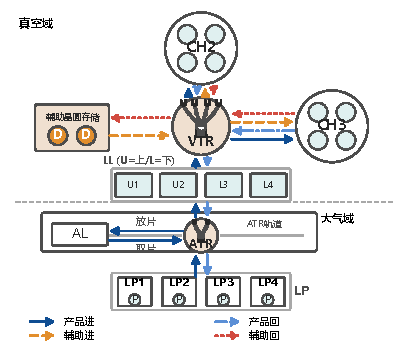
\includegraphics[width=\linewidth]{fig_system_cn_nature}
\caption{双源混流旋转腔组合设备拓扑与晶圆加工路线。}
\label{fig:system-zh-new}
\end{figure}

满片占用使产品供给与辅助晶圆复用相互制约。产品不足以填满工位时，辅助晶圆承担补位；清洁占用辅助晶圆与腔室，并改变后续可用时刻。因此，产品到达腔室并不意味着能够立即开始加工，还需满足辅助晶圆可用性、机械手服务次序和清洁边界等条件。图~\ref{fig:system-zh-new}中的两类物料路线需要在同一排程中协调。

设备采用$4\times1$并行加工与$2\times2$链式加工两种预设模式。前者由四片晶圆同步完成一次加工；后者以两片晶圆为搬运与占位单元，通过相邻周期之间的交替装卸，使每片产品连续参加两次加工。本文在两种配方均满足产品工艺要求的前提下，以相同累计名义加工时长比较运行效率。两种模式的加工周期数、辅助晶圆需求和交换次序不同，因而同一批量可能形成不同的清洁位置与完工时间。这构成本文的核心问题：在满片、驻留和共享资源约束下，如何协调两类物料与清洁动作，以及批量和清洁间隔如何改变模式选择。

已有CT研究建立了加工、搬运与吞吐率之间的解析关系\cite{perkinson1994throughput}，并通过线性规划、启发式和时间Petri网求解带驻留约束的排程\cite{rostami2002optimal,wu2010closedform,qiao2012sojourn}。研究范围进一步扩展到重入工艺、多类晶圆和可选工艺模块\cite{qiao2014revisiting,wang2020multiple,wang2025virtualcell}。四指机械手与四空间模块的稳态周期分析，以及两类晶圆投放与搬运的联合优化，为复杂设备结构提供了建模基础\cite{gu2024multifinger,yang2025miptwowafers}。有限批次还包含链首初始化、链尾退出和末批补位，辅助晶圆的返回时刻因此直接影响后续加工。

周期清洁调度采用任务序列枚举、部分装载与时刻控制、虚拟晶圆占位和腔室状态触发等方式协调清洁与生产\cite{kim2013cleaning,yu2020delay,qiao2022binary,li2022conditioncleaning}。共享缓冲同步和动态动作筛选用于避免故障停机与非周期运行中的死锁\cite{zhu2025failuredeadlock,kim2025noncyclicdeadlock}，等待约束还关系到设备产出和上游控制\cite{lee2018waiting}。对本文设备而言，清洁同时改变加工链分段、辅助晶圆占用和真空机械手次序，单独安排产品加工或清洁时刻难以完整表示这些依赖关系。

上述物料与资源约束形成混合整数调度问题。学习方法可用于直接选择CT动作，也可辅助数学规划搜索：强化学习与前瞻搜索用于非周期CT控制\cite{kim2025adaptivecluster}；在MILP中，强化学习选割、候选割排序和前瞻模仿用于选择候选不等式\cite{tang2020cut,huang2022cutranking,paulus2022looking}。HEM进一步联合决定割数量与有序割集\cite{wang2023hem}。本文沿用这一层次分解，将设备变量的结构信息用于选割，并由MILP描述工艺可行域。

本文联合建模产品供给、辅助晶圆复用、完整加工链和清洁边界，并通过配对实验分别评价排程构造与搜索策略。主要贡献如下：
\begin{enumerate}[leftmargin=*]
\item 建立双源物料流与共享资源的联合模型，描述两种预设模式下的满片加工、辅助晶圆复用与清洁动作，覆盖产品进片至回片的完整有限批次过程；
\item 构建完工时间优先的两阶段MILP，在保留第一阶段完工时间上界与主要离散次序的条件下精修等待和节拍，并量化给定PW布局下批量、清洁间隔与模式优选之间的关系；
\item 将SPBS初始化和角色感知层次割选择嵌入求解流程，通过同预算对照分别评价初始解、时间精修和选割策略对可行排程获得率与解质量的影响。
\end{enumerate}

第2节定义物料路线、工艺约束和两阶段模型；第3节介绍初始化与割选择方法；第4节分析模式选择、排程质量和求解性能；第5节给出结论。

\section{问题描述与两阶段调度模型}


\subsection{设备配置与调度任务}

给定产品批量、加工模式、晶圆配对布局和设备初始状态，调度任务是确定装载、对准、搬运、旋转、加工、清洁与回片动作的开始和结束时刻，以及共享资源上的执行次序。产品晶圆从LP出发并在加工后返回LP；辅助晶圆从真空存储区出发，完成补位或清洁任务后返回。两类路线通过机械手服务、腔室占位和辅助晶圆库存耦合。

模型输入包括动作时长、资源容量、驻留上限、清洁间隔和辅助晶圆数量。第一阶段最小化最后一片产品返回LP的时刻，第二阶段在给定完工时间上界下改善等待与加工节拍。每个可行排程表示为包含晶圆、资源及起止时刻的动作序列，用于计算运行指标并核查工艺先后与资源冲突。

模型在单次求解中采用确定性动作时长，不设置LP、对准器、装载锁、旋转腔及真空存储区以外的缓冲。等待因而对应明确的物料位置和资源占用。

\subsection{针对两种工艺模式需求的PW对建模}

为同时表示单片驻留与成对搬运，模型以晶圆对描述共享装卸和腔室占位，以单片事件描述对准与路线时间。

PW对（wafer pair）是由两个晶圆组成的物理搬运与腔室占位单元，可由“产品+产品”（产品PW对）、“辅助+辅助”（辅助PW对）或“产品+辅助”（混合PW对）构成。产品晶圆优先按模式和编号两两配对；产品数为奇数时，尾片可与一片辅助晶圆组成混合PW对，满片补位与清洁则使用辅助PW对。集合$\mathcal P^F$和$\mathcal P^L$分别索引采用两种模式的含产品PW对，包括产品PW对和必要的混合PW对。

PW对与单片事件共同描述物料动作：AL对准、产品路线和驻留时间按单片建模，双手ATR搬运、VTR成对搬运及旋转腔同步占位采用共享事件窗口。预处理给定含产品PW对的配对与兼容腔室位置，MILP在该布局内优化其余激活与分配决策、辅助晶圆身份、成对搬运、共享资源次序和事件时刻。清洁边界由清洁间隔和完整工艺段预生成，清洁激活由该布局及生产激活关系确定，具体动作时刻与生产排程联合优化。

产品晶圆沿“LP--ATR--AL--ATR--上装载锁--VTR--旋转腔--VTR--下装载锁--ATR--LP”流动，其中ATR先把晶圆放至AL完成校准，再将其取回并送入真空域；辅助晶圆从真空存储区经VTR进入旋转腔，使用结束后经VTR返回原存储区。$4\times1$模式的常规满产品批次由两个产品PW对、即四片产品晶圆组成，四个工位只执行一次同步加工，再按后装先卸顺序取出；末批产品不足时，仅在最后一个有效批次中用辅助PW对或混合PW对补齐四个工位。$2\times2$模式中，每个含产品PW对必须连续出现在相邻两个加工周期中，使其中每片产品晶圆完成两次加工。以三个产品PW对为例，链首先放入辅助PW对D，腔室自转后装入P1并完成“D+P1”腔室加工；随后交替执行腔室加工与“腔室自转+链式滑动”，占位状态依次转为“P1+P2”“P2+P3”和“P3+D”，P1、P2和P3均分别加工两次，最后再取出全部晶圆。图~\ref{fig:chain-zh}和图~\ref{fig:parallel-zh}给出两种模式的事件顺序。

\begin{figure}[t]
\centering
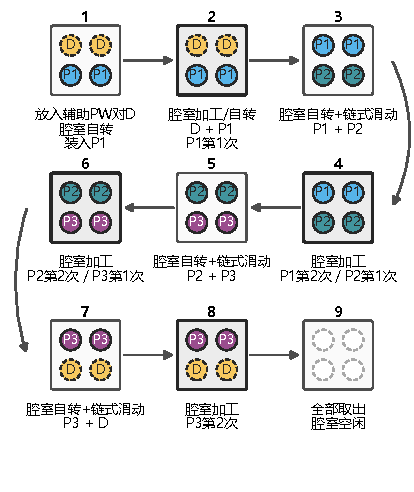
\includegraphics[width=0.99\linewidth]{fig_chain_cn_nature}
\caption{$2\times2$链式加工过程。辅助PW对D在链首与链尾用于保持腔室满片；产品晶圆随腔室旋转和链式滑动依次进入相邻加工周期，每片产品晶圆完成两次加工。}
\label{fig:chain-zh}
\end{figure}

\begin{figure}[t]
\centering
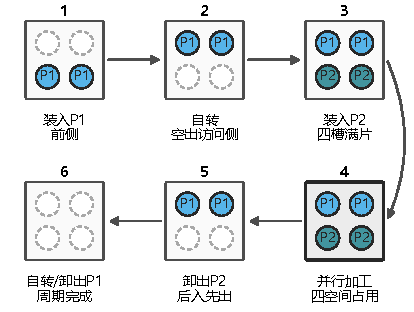
\includegraphics[width=\linewidth]{fig_parallel_cn_nature}
\caption{$4\times1$并行加工过程。两组PW对依次装入旋转腔，四个工位满片后同步加工，并按后装先卸顺序完成卸片；末批不足时由辅助晶圆补齐空余工位。}
\label{fig:parallel-zh}
\end{figure}


\subsection{源接口与基本时间关系}

表~\ref{tab:symbol-cn-a}列出集合与参数，表~\ref{tab:symbol-cn-b}列出决策变量、固定指示量与派生量。$x^F$、$x^L$和$\mu^L$取值于$[0,1]$，并由给定布局的等式约束固定为0或1。

\begin{table*}[t]
\centering
\footnotesize
\setlength{\tabcolsep}{2.5pt}
\caption{集合与参数}
\label{tab:symbol-cn-a}
\begin{tabular}{C{0.20\textwidth}C{0.20\textwidth}C{0.55\textwidth}}
\toprule
符号 & 类型与角色 & 含义 \\
\midrule
$\mathcal S,\mathcal I$ & 集合 & 物料源接口集合与物料单元集合；$i\in\mathcal I$可为产品或辅助晶圆需求。\\
$\mathcal W$ & 集合 & 产品晶圆集合，索引为$w$。\\
$\mathcal P^F,\mathcal P^L$ & 集合 & 分别采用$4\times1$和$2\times2$工艺的含产品PW对集合，索引为$p$。\\
$\mathcal C$ & 集合 & 旋转工艺腔室集合，索引为$c$。\\
$\mathcal B_c,\mathcal K_c$ & 有序集合 & 腔室$c$的$4\times1$候选批次$b$和$2\times2$产品链位置$k$。\\
$\mathcal L=\{1,2\}$ & 集合 & $4\times1$批次的前、后两侧。\\
$\mathcal Q_c,\mathcal E_c$ & 有序集合 & 腔室$c$的$2\times2$加工周期$q$与清洁区段$e$。\\
$\mathcal V_c$ & 集合 & 腔室$c$中所有$4\times1$批次与$2\times2$加工周期的并集。\\
$\mathcal O,\mathcal A$ & 集合 & 候选物理操作集合与必须满足的工艺先后弧集合。\\
$\mathcal R,\Lambda_r$ & 集合 & 共享资源集合及资源$r$的物理槽位集合。\\
$\mathcal J_c^D,\mathcal T_c$ & 集合 & 腔室$c$的辅助晶圆需求集合与可复用物理辅助晶圆集合。\\
$\chi_{is}$ & 0-1常量 & 物料单元$i$是否属于源接口$s$。\\
$\bar x^F_{pcbl},\bar x^L_{pck}$ & 0-1常量 & PW对与$4\times1$批次侧位或$2\times2$链位置的规范化对应。\\
$q_c^-(k),q_c^+(k)$ & 非负整数常量 & $2\times2$链位置$k$对应的第一次和第二次加工周期，满足$q_c^+(k)=q_c^-(k)+1$。\\
$\bar z_{ce},\bar a^F_{cbe},\bar a^L_{cqe}$ & 0-1常量 & 预生成清洁布局中的有效区段、$4\times1$批次所属区段和$2\times2$周期所属区段。\\
$H,\bar Q_c$ & 非负整数常量 & 相邻清洁间最大有效加工数，以及规范化布局生成的$2\times2$有效周期数。\\
$d_o,\delta_{oo'}$ & 非负连续常量 & 操作$o$的持续时间及先后弧$(o,o')$要求的最小间隔。\\
$d^F_\nu,d^L,r_c$ & 非负连续常量 & $4\times1$阶段$\nu$的时间、$2\times2$加工时间及腔室半周旋转时间。\\
$\rho^r_{oo'}$ & 非负连续常量 & 资源$r$从操作$o$终点空载移动或复位到$o'$起点所需时间。\\
$M,\overline R_{wr}$ & 正连续常量 & 有效大常数上界，以及晶圆$w$在受限区段$r$中的最大驻留时间。\\
$\kappa_o,\Gamma_o$ & 整数常量/集合 & 操作$o$需要的资源占用单元数及允许使用的占用单元集合。\\
$\lambda_1,\ldots,\lambda_4$ & 非负连续常量 & 第二阶段总等待、最大等待、节拍偏差和软上限超额的权重。\\
$\bar\omega_\alpha,\varepsilon_C$ & 非负连续常量 & 等待量$\alpha$的软上限与第二阶段允许的最大完工时间容差。\\
$\mathcal F,\mathcal D_{\rm fix}$ & 集合 & 完整MILP可行域，以及第二阶段固定的离散变量索引集合。\\
$\mathcal Q^w,\mathcal I_h$ & 集合 & 次级目标中的等待量，以及可计算节拍二阶差分的加工起点索引。\\
\bottomrule
\end{tabular}
\end{table*}

\begin{table*}[t]
\centering
\footnotesize
\setlength{\tabcolsep}{1pt}
\caption{决策变量与辅助变量}
\label{tab:symbol-cn-b}
\begin{tabular}{C{0.18\textwidth}C{0.15\textwidth}C{0.47\textwidth}}
\toprule
符号 & 类型与角色 & 含义 \\
\midrule
$x^F_{pcbl},x^L_{pck}$ & 连续$[0,1]$变量 & 含产品PW对是否位于$4\times1$候选侧位或$2\times2$链位置。\\
$\mu^L_{pcq}$ & 连续$[0,1]$变量 & $2\times2$含产品PW对$p$是否在腔室$c$的加工周期$q$中接受加工。\\
$u^F_{cb},f^F_{cbl},t^F_{cb}$ & 0-1二元变量 & $4\times1$批次是否启用、某侧是否用辅助晶圆补片、该批次是否为最后有效批次。\\
$u^L_{ck},a^L_c,v^L_{cq},h^L_{ck}$ & 0-1二元变量 & $2\times2$位置是否使用、腔室是否存在链、周期是否使用及该位置是否为链尾。\\
$z_{ce},a^F_{cbe},a^L_{cqe},q^{\rm cl}_{ce}$ & 0-1二元变量 & 有效清洁区段、批次或周期所属区段，以及清洁任务是否激活。\\
$\tau_{ce}$ & 0-1参数 & 区段$e$是否为恰好累计$H$个周期的最后生产区段，从而触发末端清洁。\\
$q_j,g_{j\tau}$ & 0-1二元变量 & 辅助晶圆需求是否出现，以及是否分配给物理辅助晶圆$\tau$。\\
$b_o,y^r_{oo'}$ & 0-1二元变量 & 操作$o$是否执行，以及共享资源$r$上$o$是否先于$o'$。\\
$h_{o\ell}$ & 0--1二元变量 & 操作$o$是否占用物理槽位$\ell$。\\
$\gamma_{pa}$ & 0-1二元变量 & PW对$p$在机械手路线$a$上是否采用一次成对搬运。\\
$s_o,e_o$ & 非负连续变量 & 操作$o$的开始与结束时刻。\\
$s^{F,\nu},e^{F,\nu},s^L,e^L$ & 非负连续变量 & $s_o,e_o$在$4\times1$阶段和$2\times2$周期上的具体记号。\\
$A^F_{cb},N_{ce}$ & 整数辅助变量 & $4\times1$批次的产品PW对数与清洁区段中的有效加工周期数。\\
$a_{vce}$ & 0-1二元变量 & 任务$v\in\mathcal V_c$是否属于清洁区段$e$，按任务类型取$a^F$或$a^L$。\\
$C_w,C_{\max}$ & 非负连续变量 & 产品晶圆$w$的完成时刻与批次最大完工时间。\\
$\omega_\alpha,L_{\rm sum},L_{\max}$ & 非负连续辅助变量 & 第二阶段计入的等待或空闲量、其总和与最大值。\\
$v_{ceq},\eta_\alpha$ & 非负连续辅助变量 & 加工起点二阶差分的绝对值上界和软等待上限超额。\\
$h_{ceq},\Delta_{ceq},\Phi$ & 连续辅助变量 & 加工开始时刻、可正可负的起点二阶差分，以及第二阶段线性排程质量值。\\
$\xi,\widehat\xi,\widehat C$ & 变量向量/阶段间常量 & 当前全部变量、第一阶段最好可行解及其最大完工时间。\\
\bottomrule
\end{tabular}
\end{table*}

固定参数$\chi_{is}$满足
\begin{equation}
\sum_{s\in\mathcal S}\chi_{is}=1,
\qquad i\in\mathcal I.
\label{eq:source-membership-cn}
\end{equation}
式~\eqref{eq:source-membership-cn}表示每个物料单元恰好属于一个源接口。令$|\mathcal S|=1$即可得到单源设备；令$|\mathcal S|=2$并把产品与辅助晶圆连接到不同接口，即得到本文的双源设备。

若$\mathcal A^{\rm int}$表示设备内部连接，$\mathcal A_s$表示源$s$的释放与返回连接，则
\begin{equation}
\mathcal A=\mathcal A^{\rm int}\cup
\left(\bigcup_{s\in\mathcal S}\mathcal A_s\right).
\label{eq:route-union-cn}
\end{equation}
式~\eqref{eq:route-union-cn}表示单源和双源仅在路线首尾接口上不同，内部加工、清洁、共享资源与时间约束使用同一套模型；双源物料流通过共享资源约束在同一可行域内联合求解。

两种工艺的规范化PW对位置满足
\begin{equation}
\begin{aligned}
x^F_{pcbl}&=\bar x^F_{pcbl}, &
\sum_{c,b,l}x^F_{pcbl}&=1 &&(p\in\mathcal P^F),\\
x^L_{pck}&=\bar x^L_{pck}, &
\sum_{c,k}x^L_{pck}&=1 &&(p\in\mathcal P^L).
\end{aligned}
\label{eq:pair-slot-cn}
\end{equation}
式~\eqref{eq:pair-slot-cn}表示每个PW对恰好占据一个给定的兼容位置。预设布局确定PW对的腔室、批次或链位置，模型在给定布局下优化物料复用、资源次序与连续事件时刻，最优性结论对应这一决策空间。各模式分别求解对应的调度模型，并在相同目标与工艺参数下比较。

PW对出现的位置必须启用，且同类PW对按前缀连续使用：
\begin{equation}
\begin{aligned}
x^F_{pcbl}&\le u^F_{cb}, &u^F_{c,b+1}&\le u^F_{cb},\\
x^L_{pck}&\le u^L_{ck}, &u^L_{c,k+1}&\le u^L_{ck}.
\end{aligned}
\label{eq:activation-prefix-cn}
\end{equation}
式~\eqref{eq:activation-prefix-cn}表示有产品的批次或链位置必须执行，并排除同类位置编号中的空缺。

对任一候选物理操作$o$，开始、结束和持续时间满足
\begin{equation}
0\le s_o\le Mb_o,\qquad
0\le e_o\le Mb_o,\qquad
e_o=s_o+d_ob_o.
\label{eq:operation-time-cn}
\end{equation}
式~\eqref{eq:operation-time-cn}表示未激活操作的时刻为零，激活操作持续$d_o$；该统一形式用于机械手搬运、对准、抽气、放气、旋转、产品加工、辅助晶圆搬运和清洁。

对必须依次执行的工艺弧$(o,o')\in\mathcal A$，有
\begin{equation}
b_{o'}\le b_o,\qquad
s_{o'}\ge e_o+\delta_{oo'}-M(2-b_o-b_{o'}).
\label{eq:precedence-cn}
\end{equation}
式~\eqref{eq:precedence-cn}表示后继动作只有在前驱存在时才可执行；当两者均激活时，后继必须在前驱结束并经过最小工艺间隔后开始。产品路线、辅助晶圆路线和装载--加工--卸载事件链均由该约束连接。

\subsection{两种加工模式的占位与事件顺序}

对$4\times1$模式，令$A^F_{cb}=\sum_{p,l}x^F_{pcbl}$表示批次$(c,b)$中实际分配的产品PW对数。满片与补片关系写为
\begin{equation}
\begin{aligned}
A^F_{cb}&=\sum_{p\in\mathcal P^F}\sum_{l\in\mathcal L}x^F_{pcbl},\\
\sum_{p\in\mathcal P^F}x^F_{pcbl}+f^F_{cbl}&=u^F_{cb}
&& (l\in\mathcal L),\\
\sum_{l\in\mathcal L}f^F_{cbl}&=2u^F_{cb}-A^F_{cb}.
\end{aligned}
\label{eq:full-capacity-cn}
\end{equation}
式~\eqref{eq:full-capacity-cn}表示一个有效$4\times1$批次有两个侧位，每个侧位恰好由一个产品PW对或一个辅助PW对占据；因此腔室加工开始时四个工位均被填满。

有效批次连续排列，辅助晶圆只允许出现在最后一个有效批次：
\begin{equation}
\begin{aligned}
A^F_{cb}&\ge u^F_{cb}, &u^F_{c,b+1}&\le u^F_{cb},\\
A^F_{cb}&\ge2u^F_{c,b+1},
&t^F_{cb}&\le u^F_{cb},\\
t^F_{cb}&\le1-u^F_{c,b+1},
&t^F_{cb}&\ge u^F_{cb}-u^F_{c,b+1}.
\end{aligned}
\label{eq:full-tail-cn}
\end{equation}
式~\eqref{eq:full-tail-cn}表示启用批次至少含一个产品PW对；若下一批仍启用，则当前批必须由两个产品PW对装满，不能提前使用辅助晶圆。后三个不等式使$t^F_{cb}=1$恰好标识最后一个有效批次；末个候选批次采用$t^F_{cB}=u^F_{cB}$的边界定义。

令$FL,BL,P,BU,FU$分别表示前侧装载、后侧装载、加工、后侧卸载和前侧卸载，则
\begin{equation}
\begin{aligned}
e^{F,\nu}_{cb}&=s^{F,\nu}_{cb}+d^{F}_{\nu}u^F_{cb}
\\[-1pt]&\nu\in\{FL,BL,P,BU,FU\},\\
s^{F,BL}_{cb}&\ge e^{F,FL}_{cb}+r_c-M(1-u^F_{cb}),\\
s^{F,P}_{cb}&=e^{F,BL}_{cb},\\
s^{F,BU}_{cb}&\ge e^{F,P}_{cb}-M(1-u^F_{cb}),\\
s^{F,FU}_{cb}&\ge e^{F,BU}_{cb}+r_c-M(1-u^F_{cb}).
\end{aligned}
\label{eq:full-sequence-cn}
\end{equation}
式~\eqref{eq:full-sequence-cn}表示$4\times1$批次先装前侧、旋转后装后侧，后侧装载结束即开始同步加工，随后先卸后侧、旋转、再卸前侧；$r_c$为腔室半周旋转时间。相邻批次还通过$s^{F,FL}_{c,b+1}\ge e^{F,FU}_{cb}-M(1-u^F_{c,b+1})$串行连接。

对$2\times2$模式，每个产品PW对占用一个有序链位置：
\begin{equation}
u^L_{ck}=\sum_{p\in\mathcal P^L}x^L_{pck},\qquad
u^L_{c,k+1}\le u^L_{ck},\qquad
a^L_c=u^L_{c1}.
\label{eq:mix-position-cn}
\end{equation}
式~\eqref{eq:mix-position-cn}表示链位置与产品PW对一一对应、实际位置从链首连续使用，并由$a^L_c$标识腔室$c$是否存在$2\times2$加工链。

令$q_c^-(k)$和$q_c^+(k)$分别表示链位置$k$的第一次和第二次加工周期，则PW对--周期关系为
\begin{equation}
\begin{aligned}
q_c^+(k)&=q_c^-(k)+1,\\
\mu^L_{pcq}
&=\sum_{\substack{k\in\mathcal K_c:\\q\in\{q_c^-(k),q_c^+(k)\}}}x^L_{pck},\\
\sum_{q\in\mathcal Q_c}\mu^L_{pcq}
&=2\sum_{k\in\mathcal K_c}x^L_{pck}.
\end{aligned}
\label{eq:mix-two-exposures-cn}
\end{equation}
式~\eqref{eq:mix-two-exposures-cn}把每个已分配的$2\times2$含产品PW对映射到两个相邻加工周期，且加工次数恰为2；该PW对中的每片产品晶圆继承相同的$\mu^L_{pcq}$，即使尾部采用P+D混合PW对，产品晶圆也不会漏加工。该式同时区分两种模式：$2\times2$的含产品PW对跨两个周期，$4\times1$的两个侧位PW对则在同一个满片批次中同步加工一次。

预生成布局给出腔室$c$需要的加工周期数$\bar Q_c$；链尾位置由$h^L_{ck}$识别：
\begin{equation}
\begin{aligned}
v^L_{cq}&=
\begin{cases}a^L_c,&q\le\bar Q_c,\\0,&q>\bar Q_c,
\end{cases}\\
\sum_k h^L_{ck}&=a^L_c,\qquad
h^L_{ck}\le u^L_{ck},\qquad
h^L_{ck}+u^L_{c,k+1}\le1,\\
h^L_{ck}&\ge u^L_{ck}-u^L_{c,k+1}.
\end{aligned}
\label{eq:mix-layout-cn}
\end{equation}
式~\eqref{eq:mix-layout-cn}表示含$n$个含产品PW对的连续链段需要$n+1$次加工：链首为辅助PW对+P1，内部周期为P$i$+P$i+1$，链尾为P$n$+辅助PW对；后三个关系使$h^L_{ck}$只在最后一个有效产品位置取1，末个候选位置采用$h^L_{cK}=u^L_{cK}$。

对合法链段的加工周期$(q_0,\ldots,q_T)$，令$H_0$、$B_q$和$T_0$分别表示链首装载、内部换片和链尾卸载操作，则
\begin{equation}
\begin{aligned}
e^L_{cq}-s^L_{cq}&=d^L v^L_{cq},\\
s^L_{cq_0}&=e^{H_0}_c,\\
s^{B}_{cq}&\ge e^L_{c,q-1}-M(1-a^L_c),\\
s^L_{cq}=e^{B}_{cq}\quad(q_0<q\le q_T),\\
s^{T_0}_c&\ge e^L_{cq_T}-M(1-a^L_c).
\end{aligned}
\label{eq:mix-sequence-cn}
\end{equation}
式~\eqref{eq:mix-sequence-cn}中的$H_0$表示链首辅助PW对与首个含产品PW对均完成装载的复合操作，满片条件成立后才开始首周期；每次内部换片只能在前一周期结束后执行，换片结束即开始下一周期；最后一次加工结束后才可卸出链尾。由此直接表达“辅助+P1、P1+P2、$\ldots$、Pn+辅助”的共享占位过程。

\subsection{清洁与可复用辅助晶圆}

清洁布局由$H$和完整加工边界确定，并以以下0--1指示量表示：
\begin{equation}
z_{ce}=\bar z_{ce},\qquad
a^F_{cbe}=\bar a^F_{cbe}u^F_{cb},\qquad
a^L_{cqe}=\bar a^L_{cqe}v^L_{cq}.
\label{eq:clean-layout-cn}
\end{equation}
式~\eqref{eq:clean-layout-cn}表示清洁区段的合法位置不由求解器任意选择：$4\times1$批次只能在批次边界分段，$2\times2$只能在完整链段闭合后分段；MILP仍优化这些加工和清洁任务的具体时刻。

令$N_{ce}$为区段$e$的有效加工周期数，则
\begin{equation}
\begin{gathered}
N_{ce}=\sum_b a^F_{cbe}+\sum_q a^L_{cqe},\qquad
z_{ce}\le N_{ce}\le Hz_{ce},\\
q^{\rm cl}_{ce}=z_{c,e+1}+\tau_{ce},\qquad z_{c,E_c+1}=0.
\end{gathered}
\label{eq:clean-count-cn}
\end{equation}
式~\eqref{eq:clean-count-cn}表示启用区段至少包含一次、至多包含$H$次有效加工。若存在下一个生产区段，必须激活区段间清洁；若最后一个生产区段恰好累计$H$个周期，则$\tau_{ce}=1$并激活末端清洁。两种清洁均形成完整设备动作，差别仅在于末端清洁之后没有产品加工。

把$\mathcal V_c$记为腔室$c$的$4\times1$批次和$2\times2$周期并集，$a_{vce}$为相应的$a^F$或$a^L$。对区段$e$中的任务$v$，清洁前后关系及清洁动作链为
\begin{equation}
\begin{aligned}
s_v&\ge e^{\rm cl}_{c,e-1}-M(1-a_{vce}) &&(e>1),\\
e_v&\le s^{\rm cl}_{ce}+M(1-a_{vce})+M(1-q^{\rm cl}_{ce}),\\
s^{\rm cl,BL}_{ce}&\ge e^{\rm cl,FL}_{ce}+r_c-M(1-q^{\rm cl}_{ce}),\\
s^{\rm cl,P}_{ce}&\ge e^{\rm cl,BL}_{ce}-M(1-q^{\rm cl}_{ce}),\\
s^{\rm cl,BU}_{ce}&\ge e^{\rm cl,P}_{ce}-M(1-q^{\rm cl}_{ce}),\\
s^{\rm cl,FU}_{ce}&\ge e^{\rm cl,BU}_{ce}+r_c-M(1-q^{\rm cl}_{ce}).
\end{aligned}
\label{eq:clean-time-cn}
\end{equation}
式~\eqref{eq:clean-time-cn}表示第$e$区段只能在前一次清洁完成后开始，并须在下一次清洁开始前结束。一次清洁包含两侧辅助晶圆装载、腔室旋转、清洁处理和反向卸载，其持续时间与资源占用共同约束VTR、旋转腔及四片辅助晶圆的可用时刻。

辅助晶圆需求$j$由相应物理事件激活：
\begin{equation}
q_j=
\begin{cases}
f^F_{cbl},&j\text{为$4\times1$末批补片需求},\\
a^L_c,&j\text{为$2\times2$链首或链尾需求},\\
q^{\rm cl}_{ch},&j\text{为清洁批次需求}.
\end{cases}
\label{eq:dummy-demand-cn}
\end{equation}
式~\eqref{eq:dummy-demand-cn}按末批补位、链首/链尾和清洁任务的激活状态确定辅助晶圆需求，并通过库存与复用约束分配具体晶圆。

每个有效需求必须选择一片库存中的物理辅助晶圆：
\begin{equation}
\sum_{\tau\in\mathcal T_c}g_{j\tau}=q_j,
\qquad j\in\mathcal J_c^D.
\label{eq:dummy-assign-cn}
\end{equation}
式~\eqref{eq:dummy-assign-cn}表示有效需求恰好分配一次；同一物理辅助晶圆的两次占用随后由共享资源互斥约束排序，因此只有在前一次卸载并返回存储区后才能复用。

\subsection{机械手、腔室与时间资源占用}

ATR为双手机械手、VTR为四手机械手，旋转腔内部含四个晶圆工位，其承载能力分别为2片、4片和4片。同一时刻一台ATR或VTR只能执行一个协调搬运动作，同一旋转腔也只能执行一个统一的装卸、旋转或加工阶段。因此，在资源排序层面，ATR、VTR和每个旋转腔的执行机构均建模为一个独占动作资源（单位并发资源），其双手、四手和四工位的晶圆承载能力分别由成对搬运变量、PW对以及批次/链式占位状态表达。AL同样作为独占动作资源；上、下装载锁各含两个独立物理槽位；辅助晶圆库存则把每片晶圆视为一个可复用物理身份。对需要$\kappa_o$个资源占用单元的操作$o$，有
\begin{equation}
\sum_{\ell\in\Gamma_o}h_{o\ell}=\kappa_ob_o.
\label{eq:slot-select-cn}
\end{equation}
式~\eqref{eq:slot-select-cn}表示激活操作必须获得规定数量的合法资源占用单元，未激活操作不占用资源。对于AL、ATR、VTR和旋转腔，这个“单元”是执行机构的互斥占用标记，只限制动作并发，不表示可承载的晶圆数；对于装载锁和辅助晶圆库存，则对应真实的物理槽位或物理辅助晶圆身份。

若操作$o$和$o'$可能竞争资源$r$的同一槽位$\ell$，则
\begin{equation}
\begin{aligned}
s_{o'}&\ge e_o+\rho^r_{oo'}-M(1-y^r_{oo'})
-M(1-h_{o\ell})-M(1-h_{o'\ell}),\\
s_o&\ge e_{o'}+\rho^r_{o'o}-My^r_{oo'}
-M(1-h_{o\ell})-M(1-h_{o'\ell}).
\end{aligned}
\label{eq:resource-order-cn}
\end{equation}
式~\eqref{eq:resource-order-cn}表示当两项操作竞争同一资源占用单元时，二元变量$y^r_{oo'}$必须选择一种先后顺序；$\rho^r_{oo'}$同时计入机械手空载移位或设备复位时间。该式统一用于ATR、AL、上下装载锁、VTR、旋转腔和同一片辅助晶圆，因而既禁止机械手或腔室执行机构并发执行冲突动作，也禁止物理槽位或辅助晶圆在释放前被再次使用。

上述工艺先后约束~\eqref{eq:precedence-cn}与资源排序约束~\eqref{eq:resource-order-cn}共同构成本文的死锁避免机制。对任一候选排程，把已激活操作作为节点，把工艺先后关系和求解器选择的共享资源先后关系作为有向弧；若机械手、装载锁、旋转腔或辅助晶圆之间出现循环等待，则该工艺--资源图中必然出现有向环。对于实际资源占用操作，沿环累加相应时间约束会产生正的持续时间或切换时间增量，从而要求某一操作的开始时刻严格晚于自身，违反时间可行性。因此，只有不存在循环等待、且所有物料都能沿完整路线从释放推进到返回的资源次序才能成为MILP可行解。结合装载锁槽位、旋转腔满片占位以及辅助晶圆返回后才能复用的显式建模，所建模动作中的循环等待通过时间可行性约束排除。

产品晶圆或辅助晶圆的个体阶段必须与其被选中的批次、链位置或清洁任务时间窗一致。若选择量为$x$，对应参考阶段为$[s^{\rm ref},e^{\rm ref}]$，则
\begin{equation}
\begin{aligned}
-M(1-x)&\le s_o-s^{\rm ref}\le M(1-x),\\
-M(1-x)&\le e_o-e^{\rm ref}\le M(1-x).
\end{aligned}
\label{eq:stage-link-cn}
\end{equation}
式~\eqref{eq:stage-link-cn}表示$x=1$时个体动作与其物理批次阶段同步；$x=0$时该候选对应不施加限制。它把PW对位置、产品路线、辅助晶圆需求和腔室加工窗口连接成同一时间模型。

当PW对$p$在机械手路线$a$上选择一次成对搬运时，两片晶圆的搬运阶段同步：
\begin{equation}
\begin{aligned}
-M(1-\gamma_{pa})&\le s_{w_1a}-s_{w_2a}\le M(1-\gamma_{pa}),\\
-M(1-\gamma_{pa})&\le e_{w_1a}-e_{w_2a}\le M(1-\gamma_{pa}).
\end{aligned}
\label{eq:double-transfer-cn}
\end{equation}
式~\eqref{eq:double-transfer-cn}表示$\gamma_{pa}=1$时，机械手用一次不可中断动作搬运完整PW对；$\gamma_{pa}=0$时，两片晶圆仍分别占用同一机械手并由式~\eqref{eq:resource-order-cn}排序。

对晶圆$w$进入和离开受限设备区段$r$的事件，有
\begin{equation}
0\le s_{\operatorname{out}(w,r)}-e_{\operatorname{in}(w,r)}
\le\overline R_{wr}.
\label{eq:residence-cn}
\end{equation}
式~\eqref{eq:residence-cn}表示晶圆在上装载锁、工艺腔室、下装载锁或受限制搬运区段中的物理停留时间不得超过上限，即驻留时间约束。装载锁的资源占用窗口还覆盖放片、抽气/放气、另一侧取片和压力复位。

\subsection{完工时间优先的两阶段优化}

令$C_w$为产品晶圆$w$完成下装载锁返回并回到LP的时刻，第一阶段优化目标为
\begin{equation}
C_w=e_{w,\mathrm{return}},\qquad
C_{\max}\ge C_w\ (w\in\mathcal W),\qquad
\min_{\xi\in\mathcal F}C_{\max}.
\label{eq:primary-objective-cn}
\end{equation}
式~\eqref{eq:primary-objective-cn}表示最大完工时间按最后一片产品晶圆完成完整端到端路线并返回LP的时刻计算。若清洁位于两个生产段之间，其资源占用和前后关系会推迟后续产品回片，因而自然影响$C_{\max}$；若最后一次清洁之后不再有产品加工，则该末端清洁仍保留在设备动作序列中，其完成时刻不直接作为$C_{\max}$的下界。末端清洁仍可能经共享VTR与其他腔室的产品回片竞争资源，因此其间接影响须由完整排程判定。WPH仅以产品回片的$C_{\max}$为分母。可行域$\mathcal F$由式~\eqref{eq:source-membership-cn}--\eqref{eq:residence-cn}及其对所有适用索引生成的实例约束构成。

设第一阶段得到当前最好可行解$\widehat\xi$和$\widehat C$，第二阶段固定集合$\mathcal D_{\rm fix}$中的离散结构，在最大完工时间容差内最小化线性排程质量：
\begin{equation}
\begin{gathered}
\xi_d=\widehat\xi_d\quad(d\in\mathcal D_{\rm fix}),\qquad
C_{\max}\le\widehat C+\varepsilon_C,\\
L_{\rm sum}=\sum_{\alpha\in\mathcal Q^w}\omega_\alpha,\qquad
L_{\max}\ge\omega_\alpha,\\
\Delta_{ceq}=(h_{ce,q+1}-h_{ceq})-(h_{ceq}-h_{ce,q-1}),\\
v_{ceq}\ge\Delta_{ceq},\qquad v_{ceq}\ge-\Delta_{ceq},\\
\eta_\alpha\ge\omega_\alpha-\bar\omega_\alpha,\qquad
\eta_\alpha\ge0,\\
\min\Phi=\lambda_1L_{\rm sum}+\lambda_2L_{\max}
+\lambda_3\sum_{(c,e,q)\in\mathcal I_h}v_{ceq}
+\lambda_4\sum_{\alpha\in\mathcal Q^w}\eta_\alpha.
\end{gathered}
\label{eq:secondary-objective-cn}
\end{equation}
式~\eqref{eq:secondary-objective-cn}表示第二阶段保持第一阶段获得的最大完工时间，并固定主要离散路线与资源次序，仅在保留的成对搬运选择和连续时刻上压缩总等待、最大等待与同一区段内相邻加工间隔的波动，并可对超过软等待上限的部分加罚。正式实验采用$(\lambda_1,\lambda_2,\lambda_3)=(1,10,25)$、$\varepsilon_C=10^{-6}$。软等待惩罚仅在启用对应软上限时生效；关闭该上限时不产生超额变量。限时求解以第一阶段当前最好可行值$\widehat C$作为第二阶段的完工时间上界，固定$\mathcal D_{\rm fix}$中的结构，并保留指定成对搬运变量的调整空间。

\section{结构感知MILP求解框架}

第2节的调度模型同时包含离散资源分配与连续事件时序。原始可行性要求满片占位、双源物流和共享资源次序相互协调；对偶界的收紧则依赖作用于离散选择、连续时刻及其耦合关系的有效不等式。为分别利用这两类结构，本文以结构保持二元骨架（structure-preserving binary skeleton，SPBS）构造初始可行排程，并采用\method{}选择割平面。SPBS确定可行搜索的起点，\method{}决定候选割的保留数量与加入次序，SCIP负责有效割生成、可行性检验、上下界维护和最优性证明\cite{achterberg2009scip,bestuzheva2023scip}。

求解过程依次包括初始排程构造与验证、候选割生成、保留数量预测、有序割集搜索和角色次模补全，随后继续分支定界搜索。所选割均为原模型的有效不等式，且其系数保持不变；因此，割选择影响线性松弛的收紧过程，而不改变原整数可行域。

\subsection{SPBS初始解}

SPBS首先依据配方和设备结构确定离散运行骨架，再由受限MILP求解连续事件时刻。产品晶圆按输入顺序组成PW对；$4\times1$模式PW对依次映射到腔室、批次和前后侧位，$2\times2$模式PW对按腔室轮转分配到连续链位置。批次使用、末批、链位置和末位置等激活变量随之确定。清洁计数把每个腔室的加工序列分成若干区段：$4\times1$批次进入相应清洁区间，$2\times2$链在达到清洁阈值时以辅助晶圆结束当前区段，并在清洁后用新的链首辅助晶圆继续。这样首先确定加工对象、腔室归属及允许的清洁边界，辅助晶圆的具体占用和所有连续时刻仍由模型约束完成。

在资源层，SPBS根据同一工艺路线生成保守次序。ATR先安排各腔室的$4\times1$输入和返回，并在某腔室完成其末个满片批次后尽早衔接该腔室的首个$2\times2$PW对；随后按清洁区段推进链式输入与返回。装载锁槽位采用确定性的奇偶映射破除对称，VTR次序与ATR的批次推进及清洁动作保持一致。设第$q$个松弛层级中被固定的二元变量集合为$\mathcal F_q$，骨架值为$\widehat x_j$，受限可行性子问题通过式~\eqref{eq:spbs-fix-cn}施加这些选择。

\begin{equation}
\ell_j^{(q)}=u_j^{(q)}=\widehat x_j,\qquad j\in\mathcal F_q
\label{eq:spbs-fix-cn}
\end{equation}

式~\eqref{eq:spbs-fix-cn}表示SPBS只把当前层级的骨架选择固定为变量界；开始、完成、等待等连续变量，以及该层级未固定的资源次序保持自由。

SPBS采用逐级释放固定变量的可行性搜索。五个层级对应嵌套固定集合$\mathcal F_1\supseteq\mathcal F_2\supseteq\cdots\supseteq\mathcal F_5$；在骨架值不变时，释放固定条件使受限可行域逐级扩大。若某一级未在分配预算内得到可行解，则转入下一层级。
第一层级固定产品与批次分配、激活状态、清洁区段、装载锁槽位以及ATR、AL、LL和VTR的资源次序。第二层级释放VTR次序，第三层级进一步释放装载锁次序，第四层级释放其余资源次序而保留结构分配与槽位，第五层级仅保留产品分配、激活状态和清洁区段。对于32片及以上实例，可行性搜索从第四或第五层级开始；在严格等待上限下，还考虑不附加骨架固定条件的原可行域。

各层级均求解目标为零的受限可行性子问题，并在获得首个可行解后终止。求解采用可行性优先策略、强化启发式和快速预求解，子问题阶段不添加割平面。随后，在完整模型中保留所得排程的主要离散决策与连续时刻，并补全排程稳定性相关的辅助变量。通过原模型全部约束检验的排程作为主问题的初始可行解。主问题恢复原变量界，因此其搜索范围为原模型的完整可行域。实验中的SPBS初始排程预先离线构造，并与对应模型逐一核验；PDI的积分区间和主问题的计时范围均不包含初始排程的离线构造阶段。

\subsection{HEM基线与角色感知表示}

已有学习型割选择分别以强化学习、候选割排序和前瞻模仿处理通用MILP候选集\cite{tang2020cut,huang2022cutranking,paulus2022looking}。HEM进一步指出，割选择同时包含“选哪些、选多少、按什么顺序加入”三个相互关联的决策，并用高层数量策略与低层序列策略联合处理\cite{wang2023hem}。本文保留HEM的层次分解和pointer解码框架，把HEM的13维序列模型作为直接基线，在相同训练实例、预算、随机种子、候选上限和隐藏维数下比较输入表示、解码及选后补全。HEM后续已扩展为层次序列/集合模型\cite{wang2024hemset}；本文的HEM-13D对应2023年序列模型的受控复现。

HEM基线的13维候选向量依次包含目标平行度、割有效性、归一化支撑规模、整数支撑比例、归一化违反量、割系数的均值/最大值/最小值/标准差以及目标系数的四个对应统计量。这些量能够反映当前LP点处的割质量和数值尺度，但两个有效性相近的割仍可能分别作用于离散路线变量和连续时间变量。对本文模型而言，这一区别直接对应“改变加工/资源组合”与“收紧既定组合的时序”。

在HEM的13维通用特征上，本文按变量的数学属性把变量分为二元、一般整数、目标活跃连续、连续辅助和其他五类。割$i$在角色$g$上的系数质量为
\begin{equation}
p_{ig}=\frac{\sum_{j:x_j\in g}|a_{ij}|}{\sum_j|a_{ij}|+\varepsilon}.
\label{eq:role-mass-cn}
\end{equation}
式~\eqref{eq:role-mass-cn}表示割系数绝对质量由各数学变量角色承担的比例。五个角色质量之外，新增特征还包括双边有限界变量质量、正系数质量、离散--连续耦合度$4(p_{iB}+p_{iI})(p_{iC_{\rm obj}}+p_{iC_{\rm aux}})$、最大非残余角色质量和归一化角色熵，共10维；与HEM特征合并后得到23维表示。角色划分仅取决于变量类型、目标系数和全局界，因此该表示对保持这些属性及割系数不变的变量重命名具有不变性。

HEM采用层次化“数量策略+有序子集策略”，其高层通过序列编码状态预测选割数量，低层采用LSTM编码器--解码器和pointer注意力逐项选择割\cite{wang2023hem,vinyals2015pointer}。本文在这一层次框架上构建角色感知割选择器：在候选进入LSTM之前引入角色感知分组门控编码，在pointer生成的有序序列之后加入角色次模补全，并在正式推理阶段采用宽度3的束搜索，以形成完整的RDMCT-HBS选择流程。


\subsection{角色感知编码与层次序列解码}

设第$t$次分离轮次保留的候选数为$m_t$。对候选割$i$，将23维输入写成$x_i=[x_i^{H};x_i^{R}]$，其中$x_i^{H}\in\mathbb R^{13}$为HEM通用特征，$x_i^{R}\in\mathbb R^{10}$为本文的角色特征。首先对完整向量作层归一化，再分别进行同维隐藏空间投影，并用完整23维信息生成逐维门控：
\begin{equation}
\begin{aligned}
\widetilde x_i&=\operatorname{LN}(x_i),\\
u_i^{H}&=W_H\widetilde x_i^{H}+b_H,\qquad
u_i^{R}=W_R\widetilde x_i^{R}+b_R,\\
g_i&=\sigma(W_g\widetilde x_i+b_g),\qquad
z_i=g_i\odot u_i^{H}+(1-g_i)\odot u_i^{R}.
\end{aligned}
\label{eq:gated-encoding-cn}
\end{equation}
式~\eqref{eq:gated-encoding-cn}中的$z_i\in\mathbb R^{128}$是候选割的融合嵌入。与直接把23维特征一次线性映射不同，两个投影支路分别保留通用LP质量和变量角色结构，门$g_i$再按候选自适应决定两类信息在每个隐藏维上的占比。因此，当两条割具有相近有效性但分别主要作用于离散路线变量和连续时间变量时，编码器仍可形成不同表示。该分组门控适配器是本文相对HEM输入表示的结构性改动。

融合后的候选按步骤1确定的可重复顺序输入单层LSTM：
\begin{equation}
(h_i,c_i)=\operatorname{LSTM}(z_i,h_{i-1},c_{i-1}),\qquad i=1,\ldots,m_t .
\label{eq:lstm-encoding-cn}
\end{equation}
LSTM把单条割的局部特征变为包含候选池上下文的状态$h_i$；这些状态同时服务于高层保留数量策略和低层有序选择。本文采用128维隐藏状态对排序后的候选序列进行上下文化编码，使同一候选池得到确定的编码表示，该可重复性以相同候选行及返回索引为条件；有效性同分仍由原始索引打破，因此该序列表示以有效性排序及原始索引作为确定次序的依据。

在低层第$r$个解码步，解码器根据上一时刻状态$d_r$和全部编码状态$h_i$先执行一次glimpse注意力，再计算pointer概率。记$M_{ri}$为掩码项：候选$i$若已在前缀中出现则$M_{ri}=-\infty$，否则为0，则
\begin{equation}
\begin{aligned}
a_{ri}&=v_g^\top\tanh(W_e h_i+W_d d_r)+M_{ri},\\
\alpha_{ri}&=\operatorname{softmax}_i(a_{ri}),\\
\bar h_r&=\sum_i\alpha_{ri}h_i,\\
b_{ri}&=v_p^\top\tanh(U_e h_i+U_g\bar h_r)+M_{ri},\\
P(i_r=i\mid i_{1:r-1},S_t)&=\operatorname{softmax}_i(b_{ri}).
\end{aligned}
\label{eq:pointer-decoding-cn}
\end{equation}
式~\eqref{eq:pointer-decoding-cn}说明pointer并不是给每条割独立打分：已选前缀通过解码器状态改变下一步分布，掩码保证无重复，glimpse先形成当前前缀下的候选池摘要，再由pointer产生下一条割的条件概率。该LSTM解码和pointer机制继承HEM/Pointer Network；本文改变的是其输入嵌入以及正式推理时如何搜索这一条件概率树。

训练阶段仍按策略分布随机采样以保留探索。正式推理阶段，本文不采用单一路径逐步选择，而在每一步维护$B=3$条部分序列。对父束$b=(i_1,\ldots,i_{r-1})$及其未选候选$j$，扩展分数为
\begin{equation}
L_r(b\oplus j)=L_{r-1}(b)+\log P(i_r=j\mid b,S_t),
\label{eq:beam-score-cn}
\end{equation}
随后从所有“父束$\times$候选”的扩展中保留$L_r$最大的3条。直到长度达到高层给出的$k_t$后取最高分序列。束搜索保留多个候选前缀，并以联合概率评价完整序列；随后，策略锚定的角色次模补全根据变量角色覆盖调整所选割集。

\subsection{从候选池到有序割集的逐步选择}

在第$t$次分离轮次中，算法按以下顺序工作。

\noindent\textbf{步骤1：建立候选池。} SCIP先按自身分离器生成并验证候选行$\mathcal C_t$。为控制候选状态的维数与评估成本，先按割有效性降序保留至多128个候选；有效性相同时按原始索引确定顺序，使输入池可重复。SCIP要求强制加入的割由求解器继续管理，不进入学习排序。

\noindent\textbf{步骤2：计算并编码状态。} 对候选池中的每一行提取13维HEM特征和10维角色特征，同时计算角色质量、主导角色和结构熵；随后按式~\eqref{eq:gated-encoding-cn}完成分组门控融合，并由式~\eqref{eq:lstm-encoding-cn}得到上下文化候选状态。编码后的候选集合构成$S_t$。

\noindent\textbf{步骤3：决定保留数量。} 高层策略输出经tanh限制在$[-1,1]$的动作，并映射为保留比例$\rho_t$；该比例再受全局上限0.2、SCIP本轮上限和最多16条割的数量上限共同约束，得到$k_t$。候选充足时至少保留两条，以保证每轮具有非空的候选子集。

\noindent\textbf{步骤4：逐个生成候选顺序。} 低层pointer策略在第$r$步根据$S_t$和已选前缀$i_{1:r-1}$计算剩余候选的概率，已选索引被掩码为负无穷，因而不会重复。高层数量和低层顺序的联合策略为

\begin{equation}
\pi_\theta(k_t,i_{1:k_t}\mid S_t)=\pi_\theta^H(k_t\mid S_t)
\prod_{r=1}^{k_t}\pi_\theta^L(i_r\mid S_t,i_{1:r-1}).
\label{eq:policy-cn}
\end{equation}
式~\eqref{eq:policy-cn}表示高层先给出本轮序列长度，低层再在这个长度内逐步选择不同候选；先选的割既影响随后可选集合，也通过解码器隐藏状态影响后续概率。

\noindent\textbf{步骤5：束搜索解码。} 训练时低层按概率随机采样以形成探索；测试时采用宽度3的束搜索。第$r$步把每条部分序列分别与所有未选候选连接，累加联合对数概率，再从“父束$\times$下一候选”的全部扩展中保留得分最高的3条。重复至长度$k_t$后输出最高得分序列。与逐步贪心相比，束搜索保留了早期次优但后续组合概率更高的前缀；这种有限宽神经组合搜索与神经组合优化中的束解码思想一致\cite{choo2022beam}。

\noindent\textbf{步骤6：角色次模补全。} 仅依赖联合概率的序列仍可能反复覆盖同一变量角色。算法保留pointer序列前$\lceil0.25k_t\rceil$条作为策略锚点，把其余策略顺序与按即时结构质量$q_i$排序的候选合并，并截取不超过$2k_t$条形成扩展池$\mathcal R_t$。对候选子集$S\subseteq\mathcal R_t$定义
\begin{equation}
\begin{aligned}
F_t(S)={}&\sum_{i\in S}(0.35q_i+0.20r_i)
+0.25\sum_{g\in\mathcal G}d_g\sqrt{\sum_{i\in S}p_{ig}}\\
&+\frac{0.20}{|\mathcal R_t|}\sum_{u\in\mathcal R_t}\max_{i\in S}s_{ui},
\end{aligned}
\label{eq:submodular-cn}
\end{equation}
其中$r_i$为pointer顺序归一化先验，$d_g$为扩展池中角色$g$的需求占比，$s_{ui}$为候选$u$与$i$在通用质量和角色质量上的截断余弦相似度；$q_i$综合有效性、违反量、整数支撑、可识别角色比例、主导角色比例和结构熵。式~\eqref{eq:submodular-cn}的第一项保留即时质量和学习顺序，平方根覆盖项使重复加入同一角色的边际收益递减，最后一项使所选割代表扩展池的主要结构。算法从锚点集合出发，每一步计算所有未选候选的$F_t$边际增益并加入最大者，直至达到$k_t$。在权重、角色质量与截断相似度非负并取$F_t(\varnothing)=0$时，该模块项、凹覆盖项和设施位置项构成单调次模目标。固定锚点$A_t$及扩展池后，令$f(U)=F_t(A_t\cup U)-F_t(A_t)$，则基数约束下的贪心补全对该残余目标具有标准$1-1/e$近似性质\cite{nemhauser1978analysis}。该近似比度量固定扩展池内残余代理目标的覆盖质量；PDI与求解时间由计算实验评价。

所选$k_t$条割依次按锚点原顺序和贪心补全顺序加入当前LP。候选截断、状态编码、数量预测、序列解码和次模补全共同确定本轮用于收紧线性松弛的有序割集。

\begin{table}[!htbp]
\raggedright
\footnotesize
\setlength{\tabcolsep}{3pt}
\algorithmtitle{基于并行层次REINFORCE与束搜索的割平面选择算法}
\label{alg:cut-selection-cn}
\begin{tabular}{>{\raggedright\arraybackslash}p{0.92\columnwidth}}
\toprule
\textbf{算法步骤}\\
\midrule
\textbf{输入：}SCIP已验证候选行$\mathcal C_t$、高层策略$\pi_\theta^H$、低层pointer策略$\pi_\theta^L$、束宽$B=3$、本轮求解器割上限。\\
\textbf{输出：}加入当前LP的有序割集$S_t^\star=(i_1,\ldots,i_{k_t})$。\\
\textbf{1. 训练策略。}两个采样环境并行采集以$R=-\pdi$为终端回报的求解轨迹；采用独立EMA基线的层次REINFORCE和同步Adam更新高、低层策略。正式推理时固定参数。\\
\textbf{2. 形成候选池。}按有效性降序、原始索引破同分，截取至多128行。\\
\textbf{3. 编码状态。}对每行计算13维HEM特征、10维角色特征及角色质量，经分组投影、sigmoid门控融合和LSTM编码得到候选状态。\\
\textbf{4. 确定保留数。}用$\pi_\theta^H$预测保留比例，并经0.2比例上限、SCIP上限和16条数量上限得到$k_t$。\\
\textbf{5. 初始化束。}以空序列和对数概率0初始化$\mathcal B_0$。\\
\textbf{6. 束搜索扩展。}对$r=1,\ldots,k_t$，由一次glimpse和pointer注意力得到掩码后的条件概率，将$\mathcal B_{r-1}$中的每个前缀与全部未选候选组合并累加对数概率。\\
\textbf{7. 束剪枝。}保留联合概率最高的3条父束--候选扩展得到$\mathcal B_r$；循环结束后取$\mathcal B_{k_t}$的首序列。\\
\textbf{8. 固定锚点。}保留首序列前$\lceil0.25k_t\rceil$条作为策略锚点$A_t$。\\
\textbf{9. 构造扩展池。}合并剩余pointer顺序与结构质量顺序，去重并截取至多$2k_t$条得到$\mathcal R_t$。\\
\textbf{10. 次模补全。}置$S\leftarrow A_t$；当$|S|<k_t$时，加入使$F_t(S\cup\{i\})-F_t(S)$最大的$i\in\mathcal R_t\setminus S$。\\
\textbf{11. 加入割平面。}将$S_t^\star$按锚点原顺序及补全选择顺序加入当前LP。\\
\bottomrule
\end{tabular}
\end{table}

\subsection{策略训练与精确求解}

一次SCIP限时求解构成一条求解轨迹，终端代价为该求解的PDI。当前策略在每个满足条件的割选择轮次中执行；训练以该轨迹首次有效候选集上的高层比例和低层随机序列为动作样本，并把完整求解的PDI反馈给两层策略。以$R=-\pdi$写成回报后，低层采用
\begin{equation}
\begin{aligned}
\widehat{\nabla_\theta J}
&=\frac1B\sum_{b=1}^B(R_b-\bar R_{\rm EMA})
\nabla_\theta\log\pi_\theta(\tau_b),\\
\bar R_{\rm EMA}&\leftarrow0.9\bar R_{\rm EMA}+0.1\bar R.
\end{aligned}
\label{eq:reinforce-cn}
\end{equation}
式~\eqref{eq:reinforce-cn}给出带指数移动平均基线、以首个有效候选集的动作样本构造的批量策略梯度更新；$B$为轨迹批量大小，$\tau_b$为第$b$条轨迹首次有效候选集上的采样割序列。等价地最小化以PDI为代价的优势加权对数概率，并按序列长度平均低层对数概率，防止长割序列仅因项数更多而产生过大梯度。高层使用相同PDI代价和独立EMA基线，每两轮更新一次；两层梯度范数均截断为2。训练采用并行环境采样，并在每批样本收集完成后同步更新参数，形成并行层次REINFORCE训练过程\cite{williams1992reinforce,mnih2016a3c}。

训练集含五个实例和五个随机种子。每个种子使用两个采样环境，每个采样环境每轮完成四条采用30~s时间上限和1024~MB内存上限的求解轨迹，合计八条，训练60轮；低层和高层Adam初始学习率分别为$10^{-4}$和$5\times10^{-4}$，每10轮乘0.96。训练使用随机解码，正式推理使用宽度3的束搜索。每个配置--种子组合固定使用第60轮参数，不利用基准集或测试集选择模型参数；13维HEM、23维仅特征和23维完整方法分别训练，避免把不同输入含义或补全环境的权重混用。

\method{}只排序并选择SCIP已生成的有效割，SPBS只提交经完整模型检查的可行解；二者均不改变目标、约束、整数性或界逻辑。因此，学习模块影响的是搜索路径和限时内上下界收敛速度，而可行性和最优性仍具有与默认SCIP相同的含义。

\section{计算实验与结果分析}
本文区分两类实验配置：冻结算法基准的标称并行加工及每次链式曝光均为180~s，模块驻留上限为500~s，core标称组$H=5$；模式比较使用180~s对90+90~s以及10000~s模块驻留上限。前者评价同一实例上的求解方法，不能作为相同累计加工时长的模式比较。算法基准共同采用仅根节点分离割的受控配置。

\subsection{实验设计与指标}

实验考察四个问题：批量与清洁间隔如何改变模式优选；同预算两阶段优化能否改善等待和节拍；SPBS与结构感知选割分别如何影响可行解获得率和原始--对偶收敛；规模、混流比例和参数变化如何影响求解性能。实验包括模式对照、HEM直接比较、960次SPBS配对运行、1500次等预算精修运行、300次析因运行、80次单因素扰动运行，以及各方法合计729次40--64片分布偏移运行。四张16片资源甘特图分别展示$H=10$和$H=3$下的两种纯模式。用于结果分析的可行排程均通过原模型约束检验与独立时序核算。

各对照方法采用相同的MILP、SCIP版本、实例及随机种子，并在每个比较族内使用相同时间与内存限制。设$P(t)$为最小化问题在时刻$t$的原始界，即当前最好可行目标值；$D(t)$为对偶界，即搜索树给出的全局下界。进一步记$\Delta(t)=|P(t)-D(t)|$、$m(t)=\min\{|P(t)|,|D(t)|\}$和$M(t)=\max\{|P(t)|,|D(t)|\}$。当两界有限、同号且不相等时，按照SCIP的定义，终止相对原始--对偶间隙为：
\begin{equation}
G_{\rm end}=100\,\frac{\Delta(T)}{m(T)}.
\label{eq:terminal-gap-cn}
\end{equation}
若两界相等，SCIP令$G_{\rm end}=0$；若两界异号或有效界尚未同时获得，则返回$+\infty$。式~\eqref{eq:terminal-gap-cn}以两界绝对值中的较小者归一化，因此$G_{\rm end}$不以100\%为上限；超过100\%表示上下界绝对差大于两界绝对值中的较小者。

SCIP计算PDI时采用另一种有界归一化。记瞬时积分gap为
\begin{equation}
g_{\rm PDI}(t)=100\,\frac{\Delta(t)}{M(t)},\qquad
\pdi=\int_0^T g_{\rm PDI}(t)\,\mathrm dt.
\label{eq:pdi-gap-cn}
\end{equation}
式~\eqref{eq:pdi-gap-cn}适用于有限同号且不相等的两界；两界相等时SCIP令$g_{\rm PDI}(t)=0$，其余情形令$g_{\rm PDI}(t)=100$。因此瞬时积分gap始终位于$[0,100]$，PDI越低表示越早缩小界差。PDI为0要求gap在几乎整个计时窗内为0；$G_{\rm end}=0$只表示运行结束时证明最优，而PDI还计入最优性证明之前的界差。两项指标均采用SCIP的定义与求解统计量\cite{achterberg2009scip,bestuzheva2023scip}。

制造实例是推断单位：先在实例内聚合随机重复，再对配对实例差异计算非参数95\% bootstrap区间和Wilcoxon符号秩检验，并在预设分析族内作Holm校正。限时运行保留在汇总中，避免把随机种子误当成独立制造证据。

表~\ref{tab:gantt-config-zh}给出16片代表性甘特图对应的实验参数。两台旋转腔共享VTR，产品晶圆和辅助晶圆沿各自路线竞争机械手、load lock和腔室空间；清洁计数、旋转及搬运时间均进入同一MILP。图示排程均通过SCIP原模型约束检验和独立时序核算，用于比较两种模式的资源占用与事件衔接。

表~\ref{tab:gantt-config-zh}中的数值定义计算实验配置。产品回片时间比较采用相同累计名义加工时长：$4\times1$为一次180~s，$2\times2$为两次90~s。配方满足产品工艺要求作为比较前提，实验评价排程性能。

\begin{table*}[!htbp]
\centering
\footnotesize
\setlength{\tabcolsep}{2pt}
\caption{清洁频率模式实验与代表甘特图的实验参数（等总名义加工时间场景）。}
\label{tab:gantt-config-zh}
\begin{tabular}{C{0.10\textwidth} C{0.29\textwidth} C{0.10\textwidth} C{0.29\textwidth}}
\toprule
类别 & 参数与取值 & 类别 & 参数与取值\\
\midrule
旋转腔 & CH2、CH3，两台共享旋转PM，每台4个空间 & 工艺时间 & $4\times1$为180~s；$2\times2$为90+90~s\\
清洁 & 相邻清洁间最多$H=3$--10个有效加工周期；纯辅助晶圆清洁500~s & 腔室动作 & 旋转180$^\circ$为2~s；相邻腔室动作间隔1~s\\
ATR & 1台双手机器人，容量2；装/卸4~s，完整带片搬运11~s & VTR & 1台四手机器人，容量4；带片搬运4~s，空载换位4~s\\
ATR细节 & LL--LP空载返回6~s；AL处PW对交换8~s & AL & 容量1；每片最小对准占用20~s\\
Load lock & LLupper每槽抽气/复位30~s，LLlower每槽放气/复位25~s & LL容量 & upper和lower各含2个独立槽位\\
物料源 & LP1--LP4，每个容量25片 & 辅助晶圆 & 可复用8片，每腔4片；存储区容量10片\\
批次与模型 & 产品基本批量4片；13个工艺步骤 & 腔室容量界 & 每台PM最多15个$4\times1$批次槽\\
模型上界 & Big-$M=10000$；模块和机器人驻留上界均为10000~s & 等待设置 & 可避免等待硬上限取0，表示关闭该可选限制\\
求解目标 & 产品回片完工时间与等待精修 & 策略 & 固定训练种子1、第60轮、23维特征\\
解码与割池 & 束宽3；候选割池128，单轮最多选16条 & 求解器 & SCIP随机种子1；采用可用且通过验解的初始排程\\
求解与选图 & 产品回片目标；模式比较采用完工时间界；甘特图采用等待精修后的排程 & 排程验证 & 所有排程均通过原模型及独立验解\\
\bottomrule
\end{tabular}
\end{table*}

\subsection{清洁触发位置与批量驱动的工艺模式选择}

多空间CT的稳态研究通常以周期或吞吐率评价设备效率\cite{gu2024multifinger}。本文针对有限批次，以最后一片产品晶圆返回LP的时刻定义$C_{\max}$，并以$\mathrm{WPH}=3600|\mathcal W|/C_{\max}$表示等效批次产出率。纯$4\times1$每片加工180~s，纯$2\times2$每片加工90+90~s，1:1混跑按晶圆所属模式使用相应配方。$H$计量每腔相邻清洁间的满片加工周期数，$4\times1$批次计1次，$2\times2$的每次曝光各计1次。模型按周期上限和完整链边界构造加工区段，并计入500~s清洁及其辅助晶圆装卸、旋转和搬运。

表~\ref{tab:mode-extended-zh}给出$H=3$和10的模式比较，表~\ref{tab:clean-crossover-zh}汇总$H=3$--10的逐点结果。其中$H=4$--9实验包含36个配置，训练与求解器种子均为1，每例主求解上限14400~s，关闭第二阶段；36个排程均通过独立验解，其中35个证明最优。16片、$H=5$、纯$2\times2$在该预算内获得907~s可行解；以此为初始排程，对同一实例追加28800~s独立求解后，可行上界降至898~s，下界为694~s，终止gap为29.39\%。新排程通过主模型复验与4~s交换检查。该延长预算实验用于确定模式比较中的可行上界，其计算时间不计入固定预算的算法性能比较。清洁未激活时，16片纯$2\times2$在$H=6$--10下生成相同的MILP，最优完工时间均为898~s。

\begin{table*}[!htbp]
\centering
\footnotesize
\setlength{\tabcolsep}{4pt}
\caption{相同累计名义加工时长下的清洁端点比较。清洁总次数为两台腔室的内部与末端清洁次数之和。 $\dagger$表示经验证的完工时间上界；相应WPH按该完工时间计算。}
\label{tab:mode-extended-zh}
\begin{tabular}{cccccc}
\toprule
批次（片） & $H$ & 模式 & 清洁总次数 & $C_{\max}$（s） & WPH（片/h）\\
\midrule
8 & 10 & 纯$4\times1$ & 0 & 610 & 47.21\\
8 & 10 & 纯$2\times2$ & 0 & \textbf{578} & \textbf{49.83}\\
8 & 10 & 4:4混跑 & 0 & 654 & 44.04\\
8 & 3 & 纯$4\times1$ & 0 & 610 & 47.21\\
8 & 3 & 纯$2\times2$ & 2 & \textbf{578} & \textbf{49.83}\\
8 & 3 & 4:4混跑 & 1 & 654 & 44.04\\
\midrule
16 & 10 & 纯$4\times1$ & 0 & 944 & 61.02\\
16 & 10 & 纯$2\times2$ & 0 & \textbf{898} & \textbf{64.14}\\
16 & 10 & 8:8混跑 & 0 & 939 & 61.34\\
16 & 3 & 纯$4\times1$ & 0 & \textbf{944} & \textbf{61.02}\\
16 & 3 & 纯$2\times2$ & 4 & 1402 & 41.08\\
16 & 3 & 8:8混跑 & 2 & 1530 & 37.65\\
\midrule
24 & 10 & 纯$4\times1$ & 0 & 1268 & 68.14\\
24 & 10 & 纯$2\times2$ & 0 & $\mathbf{1237}^{\dagger}$ & \textbf{69.85}\\
24 & 10 & 12:12混跑 & 0 & 1250 & 69.12\\
24 & 3 & 纯$4\times1$ & 2 & \textbf{1268} & \textbf{68.14}\\
24 & 3 & 纯$2\times2$ & 6 & $2220^{\dagger}$ & 38.92\\
24 & 3 & 12:12混跑 & 4 & $2324^{\dagger}$ & 37.18\\
\bottomrule
\end{tabular}
\end{table*}

\begin{table*}[tp]
\centering
\footnotesize
\setlength{\tabcolsep}{3pt}
\caption{给定PW对布局下，8、16和24片批次在$H=3$--10下的三模式完工时间、清洁次数与优选模式。时间单位为s。}
\label{tab:clean-crossover-zh}
\begin{tabular}{cccccccccc}
\toprule
\multirow{2}{*}{批次（片）} & \multirow{2}{*}{$H$} & \multicolumn{3}{c}{$C_{\max}$（s）} & \multirow{2}{*}{$\Delta C_{\max}$（s）} & \multicolumn{3}{c}{清洁总次数} & \multirow{2}{*}{优选模式}\\
\cmidrule(lr){3-5}\cmidrule(lr){7-9}
 & & 纯$4\times1$ & 纯$2\times2$ & 1:1混跑 & & 纯$4\times1$ & 纯$2\times2$ & 1:1混跑 & \\
\midrule
8 & 3 & 610 & 578 & 654 & -32 & 0 & 2 & 1 & 纯$2\times2$\\
8 & 4 & 610 & 578 & 654 & -32 & 0 & 0 & 0 & 纯$2\times2$\\
8 & 5 & 610 & 578 & 654 & -32 & 0 & 0 & 0 & 纯$2\times2$\\
8 & 6 & 610 & 578 & 654 & -32 & 0 & 0 & 0 & 纯$2\times2$\\
8 & 7 & 610 & 578 & 654 & -32 & 0 & 0 & 0 & 纯$2\times2$\\
8 & 8 & 610 & 578 & 654 & -32 & 0 & 0 & 0 & 纯$2\times2$\\
8 & 9 & 610 & 578 & 654 & -32 & 0 & 0 & 0 & 纯$2\times2$\\
8 & 10 & 610 & 578 & 654 & -32 & 0 & 0 & 0 & 纯$2\times2$\\
\midrule
16 & 3 & 944 & 1402 & 1530 & 458 & 0 & 4 & 2 & 纯$4\times1$\\
16 & 4 & 944 & 1470 & 939 & 526 & 0 & 2 & 2 & 1:1混跑\\
16 & 5 & 944 & 898$^{\dagger}$ & 939 & -46 & 0 & 2 & 0 & 纯$2\times2$\\
16 & 6 & 944 & 898 & 939 & -46 & 0 & 0 & 0 & 纯$2\times2$\\
16 & 7 & 944 & 898 & 939 & -46 & 0 & 0 & 0 & 纯$2\times2$\\
16 & 8 & 944 & 898 & 939 & -46 & 0 & 0 & 0 & 纯$2\times2$\\
16 & 9 & 944 & 898 & 939 & -46 & 0 & 0 & 0 & 纯$2\times2$\\
16 & 10 & 944 & 898 & 939 & -46 & 0 & 0 & 0 & 纯$2\times2$\\
\midrule
24 & 3 & 1268 & 2220$^{\dagger}$ & 2324$^{\dagger}$ & 952 & 2 & 6 & 4 & 纯$4\times1$\\
24 & 4 & 1268 & 2928$^{\dagger}$ & 1827$^{\dagger}$ & 1660 & 0 & 4 & 2 & 纯$4\times1$\\
24 & 5 & 1268 & 1769$^{\dagger}$ & 1796 & 501 & 0 & 2 & 2 & 纯$4\times1$\\
24 & 6 & 1268 & 1880$^{\dagger}$ & 1263$^{\dagger}$ & 612 & 0 & 2 & 1 & 1:1混跑\\
24 & 7 & 1268 & 1237$^{\dagger}$ & 1250 & -31 & 0 & 2 & 0 & 纯$2\times2$\\
24 & 8 & 1268 & 1237$^{\dagger}$ & 1250 & -31 & 0 & 0 & 0 & 纯$2\times2$\\
24 & 9 & 1268 & 1237$^{\dagger}$ & 1250 & -31 & 0 & 0 & 0 & 纯$2\times2$\\
24 & 10 & 1268 & 1237$^{\dagger}$ & 1250 & -31 & 0 & 0 & 0 & 纯$2\times2$\\
\bottomrule
\end{tabular}
\par\smallskip
\parbox{0.95\textwidth}{\footnotesize 清洁总次数为两台腔室内部与末端清洁之和。$\dagger$表示可行上界，其余完工时间已证明最优。$\Delta C_{\max}$为表列纯$2\times2$与纯$4\times1$时间之差。优选模式由最优值比较或可行上界低于竞争模式下界确定。}
\end{table*}

8片批次在$H=3$--10下的三模式完工时间分别保持610、578和654~s，纯$2\times2$较纯$4\times1$缩短5.25\%。$H=3$时纯$2\times2$与混跑分别产生2次和1次末端清洁；$H\ge4$时均无清洁。该批量未形成内部清洁，模式排序在所测清洁间隔内保持一致。

16片批次的优选模式随清洁间隔变化。$H=3$时，纯$2\times2$和混跑各含2次内部清洁，纯$4\times1$以944~s最优。$H=4$时，纯$2\times2$仍含2次内部清洁，混跑仅含2次末端清洁，以939~s优于纯$4\times1$的944~s。$H=5$时，纯$2\times2$只产生2次末端清洁，其898~s可行排程优于另外两种模式的最优值，纯模式优先顺序由$H=4$的$4\times1$切换为$H=5$的$2\times2$。$H=6$--10时三模式均无清洁，纯$2\times2$以898~s最优，较纯$4\times1$和混跑分别缩短4.87\%和4.37\%。

这一变化由完整链分段和清洁位置共同驱动。16片纯$2\times2$每腔包含4个产品PW对；$H=3$按2+2个PW对分段，$H=4$按3+1分段，$H\ge5$可形成一条完整链。因此，$H=3$和4虽然内部清洁数相同，仍具有不同的供片与回片次序；$H=4$的1470~s对应后一分段布局。模式选择需要同时匹配批量、配方构成和允许的完整链长度。实验采用随$H$重构的预设完整链布局，因此表中比较反映清洁上限与链布局的联合效应。

24片批次的扩展实验覆盖$H=3$--6及三种预设模式，每个配置的主求解预算为7200~s。纯$4\times1$在四个清洁间隔下的最优完工时间均为1268~s。$H=4$时，纯$2\times2$与混跑的求解下界分别为1342和1774~s；$H=5$时，纯$2\times2$的下界为1440~s，混跑的最优值为1796~s，因此这两个清洁间隔均由纯$4\times1$优选。$H=6$时，混跑取得1263~s可行排程，低于纯$4\times1$的最优值1268~s及纯$2\times2$的下界1440~s，确定了混跑的模式优势；混跑自身的终止gap为10.40\%。$H=3$的纯$2\times2$配置经28800~s独立求解，得到2220~s可行排程、2082~s下界和6.63\%终止gap。该排程通过主模型复验及4~s交换检查；其下界与混跑下界2302~s均高于纯$4\times1$的最优值1268~s，因而$H=3$也由纯$4\times1$优选。延长预算的求解用于模式排序判定，运行时间不纳入原固定预算的算法比较。由此，24片批次在$H=3$--5时优选纯$4\times1$，在$H=6$时优选1:1混跑。与16片结果相比，24片批次在$H=5$时的优选模式由纯$2\times2$变为纯$4\times1$，说明清洁间隔的模式选择效应取决于批量与完整链布局。

24片$H=7$--10的12个配置均获得通过验解的排程。对$H=10$混跑的独立求解在28800~s预算内证明最优完工时间为1250~s；$H=7$--10的混跑MILP的目标、约束与变量界完全相同，因此四个清洁间隔对应相同的最优完工时间。纯$2\times2$在$H=8$--10下具有1237~s可行排程；将其生产事件时序迁移至$H=7$模型，并安排两次末端清洁后，同样得到经原模型复验的1237~s排程。纯$2\times2$在$H=7$及$H=8$--10下的有效界区间分别为$[712,1237]$和$[842,1237]$~s。其可行上界均低于混跑的1250~s与纯$4\times1$的1268~s最优值，因此$H=7$--10均优选纯$2\times2$，所构造排程较两种竞争模式分别缩短1.04\%和2.44\%。延长预算求解与排程迁移用于模式判定，其计算时间独立于固定预算的算法比较。

四张资源甘特图均采用16片批次，分别展示$H=10$和3的两种纯模式。各图横轴截至最后一片产品返回时刻$C_{\max}$；纯$4\times1$每次加工180~s，纯$2\times2$每次曝光90~s。为分析最短完工时间排程的等待分布，$H=10$纯$2\times2$在保持$C_{\max}\le898+10^{-6}$~s的条件下进一步最小化路线总等待，并允许调整资源次序；所得最优路线总等待为492~s。路线等待按每片晶圆六个相邻工序间隔累计，其中AL成对协调占448~s、加工后卸片前等待占36~s、下装载锁回片前等待占8~s。该路线指标统计工序间等待，腔室内两次加工之间的间隔另行计量。

图中腔室泳道将交换动作与等待分开绘制：灰色交换块按实际动作起止时刻绘制，额外等待以浅粉色表示。相邻加工间隔由交换前等待与交换过程共同构成。四指VTR的合并交换耗时4~s；拆分交换包含4~s卸片、至少4~s空载换位及4~s装片，并允许在卸片与装片之间协调其他物料动作。图~\ref{fig:gantt-cleanH10-22-zh}中CH2首次相邻加工间隔为63~s，其中59~s为交换前等待，4~s为合并交换。该排程中，下一产品PW对W5/W6在299~s进入上装载锁，329~s完成真空侧准备；CH2于270~s结束前一周期后等待至329~s，再执行329--333~s的合并交换。$H=3$的短链排程中，多数相邻周期采用连续4~s合并交换；CH2第五、六周期之间包含1106--1108~s和1112--1116~s两段等待，以及1108--1112~s卸片和1116--1120~s装片。末次加工在装片完成的1120~s立即开始，至1210~s结束。两种排程均保持每次加工90~s。进一步在同一$H=10$模型中将两个腔室全部8个相邻加工间隔限制为4~s，得到经独立验解的最优完工时间960~s，比898~s增加62~s（6.90\%）。连续交换压缩了局部加工间隔，同时约束了共享资源的供回片次序；在该有限批次下，允许局部等待获得更短的整批完工时间。

\begin{figure}[!t]
\centering
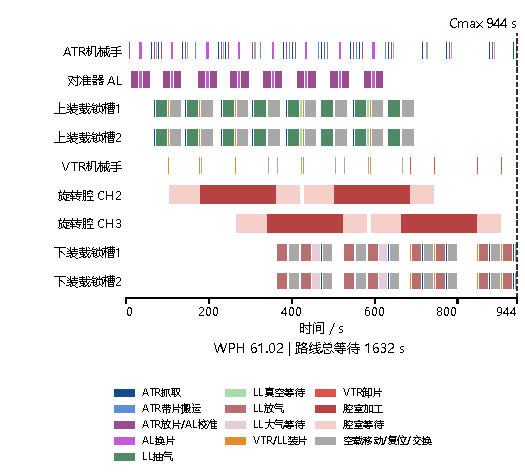
\includegraphics[width=\linewidth]{fig_resource_gantt_cleanH10_w16_41_cn_nature}
\caption{$H=10$时16片纯$4\times1$排程。无清洁，$C_{\max}=944$~s，WPH为61.02片/h，路线累计等待为1632~s。}
\label{fig:gantt-cleanH10-41-zh}
\end{figure}

\begin{figure}[!t]
\centering
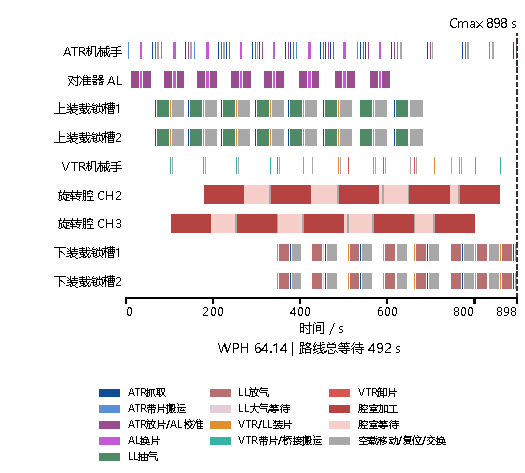
\includegraphics[width=\linewidth]{fig_resource_gantt_cleanH10_w16_22_cn_nature}
\caption{$H=10$时16片纯$2\times2$的等待精修排程。无清洁，$C_{\max}=898$~s，WPH为64.14片/h；在该完工时间约束下，路线累计等待最小值为492~s。腔室泳道中灰色表示4~s交换动作，浅粉色表示等待。}
\label{fig:gantt-cleanH10-22-zh}
\end{figure}

\begin{figure}[!t]
\centering
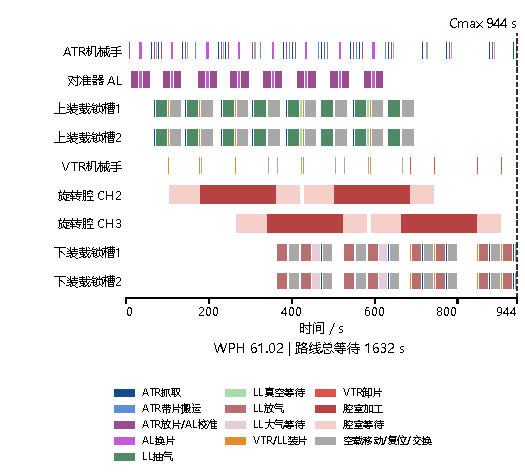
\includegraphics[width=\linewidth]{fig_resource_gantt_cleanH3_w16_41_cn_nature}
\caption{$H=3$时16片纯$4\times1$排程。$C_{\max}=944$~s，WPH为61.02片/h，路线累计等待为1632~s。}
\label{fig:gantt-cleanH3-41-zh}
\end{figure}

\begin{figure}[!t]
\centering
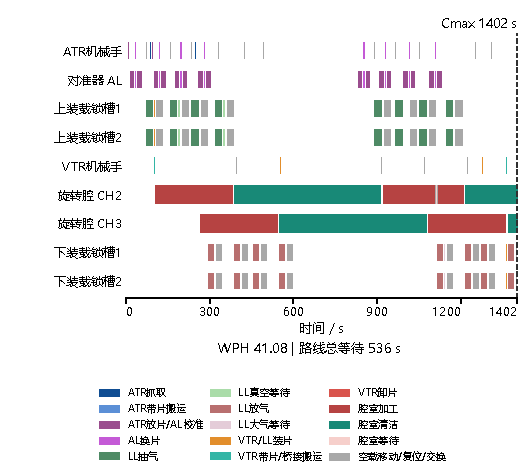
\includegraphics[width=\linewidth]{fig_resource_gantt_cleanH3_w16_22_cn_nature}
\caption{$H=3$时16片纯$2\times2$排程。包含2次内部清洁和2次末端清洁；图示时域截至产品回片，$C_{\max}=1402$~s，WPH为41.08片/h，路线累计等待为536~s；腔室泳道中交换动作与等待分别绘制。}
\label{fig:gantt-cleanH3-22-zh}
\end{figure}


\subsection{等预算下的等待与节拍精修}

等待时间约束会进一步影响制造系统的产出和控制表现\cite{lee2018waiting}。同为600~s总预算时，完整两阶段工作流采用540~s主求解加至多60~s精修，单阶段对照将600~s全部用于主求解。图~\ref{fig:workflow-zh-new}显示，两阶段工作流的路线总等待、最大等待、节拍变异系数和节拍偏差分别降低51.91\%、68.89\%、39.70\%和94.05\%，四项实例级配对差异经Holm校正后均显著，表明两阶段工作流能够在相同总预算下明显改善排程等待与节拍质量。

二次目标对照与完整线性精修均使用540+至多60~s。线性精修的节拍偏差为22.04，较二次目标的60.18降低63.38\%，该配对差异经Holm校正后显著（$p=0.0377$）；路线总等待、最大等待和节拍变异系数整体接近。在相同预算下，线性精修显著降低了所定义的节拍偏差。

\begin{figure}[!htbp]
\centering
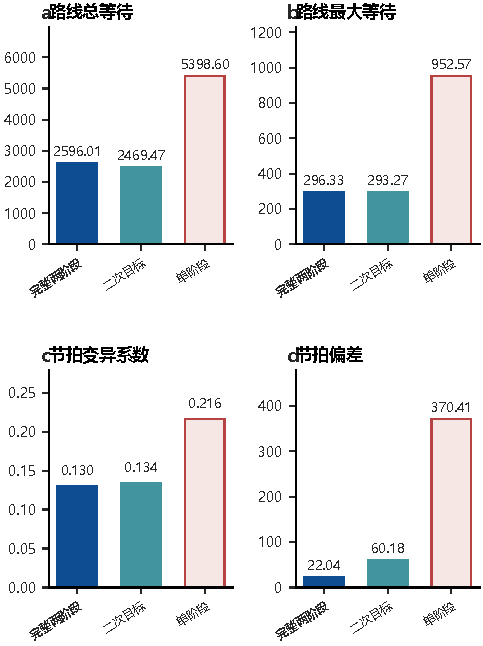
\includegraphics[width=\linewidth]{fig04_workflow_cn_nature}
\caption{相同600~s总预算下的排程运行质量。（a）路线总等待时间；（b）路线最大等待时间；（c）节拍变异系数；（d）节拍偏差。三种配置采用相同的20个实例，每种500次运行；纵轴单位依次为s、s、无量纲和s，柱顶为观察均值。}
\label{fig:workflow-zh-new}
\end{figure}
表~\ref{tab:refinement-ablation-zh}分离第二阶段及精修目标形式的影响，与表~\ref{tab:spbs-zh-new}的初始化消融共同评价工作流组件。

\begin{table*}[!htbp]
\centering\footnotesize
\setlength{\tabcolsep}{3pt}
\caption{第二阶段及目标形式消融。每个配置包含20个实例、500次运行，总预算均为600~s；表中为实例聚合均值，各指标越小越好。}
\label{tab:refinement-ablation-zh}
\begin{tabular}{ccccc}
\toprule
配置 & 总等待（s） & 最大等待（s） & 节拍CV & 节拍偏差（s）\\
\midrule
完整线性精修 & 2596.01 & 296.33 & 0.130 & 22.04\\
二次目标精修 & 2469.47 & 293.27 & 0.134 & 60.18\\
移除第二阶段 & 5398.60 & 952.57 & 0.216 & 370.41\\
\bottomrule
\end{tabular}
\end{table*}


\subsection{SPBS与结构感知割选择}

表~\ref{tab:spbs-zh-new}汇总SPBS配对实验，包含48个实例、每个实例10个配对种子。计时比较评价离线SPBS构造完成后的主求解性能。相对无初始解条件，预计算SPBS将可行解获得率由51.67\%提高至100\%，增加48.33个百分点（95\%区间$[34.58,62.29]$）；平均PDI由27473.05降至20278.78，降低7194.27或26.19\%（95\%区间$[5145.78,9317.61]$）。两项配对差异经Holm校正后仍显著（$p=2.55\times10^{-5}$和$p=3.46\times10^{-8}$）。预计算SPBS提高了后续求解阶段的可行排程获得率，并改善原始--对偶收敛。

\begin{table}[!htbp]
\centering
\footnotesize
\setlength{\tabcolsep}{3pt}
\caption{预计算SPBS对限时MILP搜索的影响，计时不含初始解构造。每个条件包含48个实例、每例10个配对种子，共480次运行。}
\label{tab:spbs-zh-new}
\begin{tabular}{cccc}
\toprule
指标 & 无初始解 & SPBS & 观察变化\\
\midrule
可行解获得率（\%） & 51.67 & 100.00 & +48.33个百分点\\
平均PDI & 27473.05 & 20278.78 & -26.19\%\\
\bottomrule
\end{tabular}
\end{table}

HEM-13D是与本文结构感知割选择器最直接的学习型基线。两者共享同一SPBS、训练实例、随机种子、候选上限、隐藏维数和600~s求解预算，每种方法包含500次运行。表~\ref{tab:hem-direct-zh}给出两种策略的配对比较。相对HEM-13D，\method{}的平均PDI由16823.18降至16585.70，平均求解时间由219.65~s降至218.32~s，平均终止相对gap由127.24\%降至126.01\%，证明最优率由62.4\%提高到63.2\%；完整方法的500次运行均获得可行解。按20个制造实例聚合随机重复后，四项配对均值差的95\% bootstrap区间均包含0，Holm校正$p$值均为1.0。相同SPBS条件下，两种学习策略的观察均值接近；配对检验结果为这些均值变化提供了统计解释。

\begin{table}[!htbp]
\centering
\footnotesize
\caption{共同SPBS和预算下\method{}相对HEM-13D的直接比较。}
\label{tab:hem-direct-zh}
\begin{tabular}{cccc}
\toprule
指标 & HEM-13D & \method{} & 观察变化\\
\midrule
平均PDI & 16823.18 & 16585.70 & -1.41\%\\
平均求解时间（s） & 219.65 & 218.32 & -0.61\%\\
平均终止gap（\%） & 127.24 & 126.01 & -0.97\%\\
证明最优率（\%） & 62.4 & 63.2 & +0.80个百分点\\
\bottomrule
\end{tabular}
\end{table}

该对照在相同初始化和求解预算下联合评价角色感知表示、序列解码与结构补全，量化其在共同SPBS条件下对PDI、求解时间、终止间隙和证明最优率的影响。

\subsection{规模、混流构成与求解难度}

析因设计包含$4\times5\times3=60$个晶圆数--配方构成--加工尺度单元，每个单元使用5个求解器种子，共300次运行。图~\ref{fig:doe-zh-new}显示明显的规模转折：8片和16片各自的75次运行均证明最优，平均PDI分别为28.13和1876.54，平均求解时间为0.34和33.86~s；24片和32片的证明最优率降至36\%和20\%，平均PDI升至31155.94和32959.89，平均求解时间升至408.55和433.20~s。

预设PDI析因模型的$R^2=0.998$。在$1{:}1$混跑条件下，24片和32片的附加交互系数分别为37729.48和40788.63，而加工尺度主效应及其预设交互项的95\%区间均包含0。因此，在所测0.9--1.1加工尺度范围内，求解难度主要由批次规模与混流构成的交互驱动，加工尺度的影响相对较小。

\begin{figure}[!htbp]
\centering
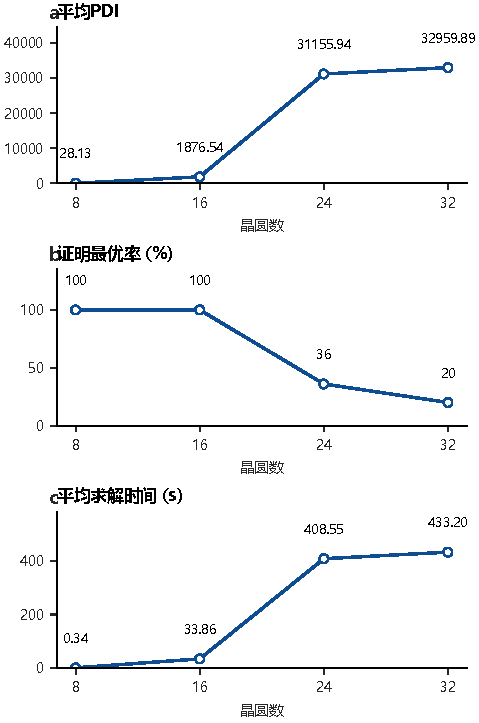
\includegraphics[width=\linewidth]{fig05_doe_cn_nature}
\caption{批次规模对求解性能的影响。（a）平均PDI；（b）证明最优率；（c）平均求解时间。横轴为晶圆数（片），纵轴单位依次为PDI、\%和s；每个规模包含75次运行，共300次运行。}
\label{fig:doe-zh-new}
\end{figure}

\subsection{参数扰动下的可运行性}

既有研究表明，清洁动作及其触发条件会改变CT的机器人动作序列、周期时间和晶圆延迟\cite{yu2020delay,li2022conditioncleaning}。据此，单因素敏感性实验覆盖搬运、加工、清洁间隔和真空区辅助晶圆库存的8个预设场景，共80次运行。全部运行均获得并验解可行排程，其中20次证明最优；场景平均PDI位于28899.41--42478.32之间。较长清洁间隔对应最低平均PDI，较慢搬运对应最高平均PDI，反映了所测参数配置下平均搜索表现的差异。

\subsection{分布偏移下的可行排程交付}

分布偏移测试把批次扩大到40--64片并改变混流组成，9个制造场景中全部对照方法共形成729次运行，其中完整方法为135次。该实验评价规模与混流组成变化下的排程交付和求解效率。全部729次运行均返回通过原模型约束检验与独立时序核算的可行排程，说明共享SPBS--MILP--SCIP链路在所测规模与配方构成变化下持续输出可验证的排程。该组证明最优率为0\%；完整方法、默认SCIP和自适应评分方法的平均PDI分别为73919.15、73670.99和70915.54。可行排程交付在该组保持100\%，平均PDI则以自适应评分方法最低。

\subsection{模式选择与求解性能的讨论}

模式优选取决于清洁在有限批次中的位置。内部清洁延迟后续加工链，而末端清洁对产品回片目标的影响不同。16片批次在$H=4$时由混合模式优选，24片批次的相应优选区间移至$H=6$，说明仅依据单周期加工能力或清洁间隔无法确定有限批次的优选模式，还需考虑批量与完整链布局。

模式优选可以由可行上界与竞争模式的下界直接确定。24片、$H=7$--10时，纯$2\times2$的1237~s可行上界低于另外两种模式的最优值，因此在所比较布局下优选纯$2\times2$。模式对照确定批量与清洁条件下的工艺选择，同预算算法对照则量化搜索性能。

各求解环节对应不同的排程性能指标。预计算SPBS提高后续限时搜索的可行解获得率，两阶段精修改善等待与节拍；共同SPBS下，完整选割策略与HEM的观察平均指标接近。规模扩展实验的可行排程获得率为100\%，自适应评分取得最低的观察平均PDI。这些结果分别量化了排程可获得性、时间质量和界收敛表现。

\section{结论}

本文研究双源混流PECVD旋转腔设备的有限批次调度。产品与辅助晶圆通过PW对连接两条物料路线，两阶段MILP联合描述满片加工、辅助晶圆复用、周期清洁、驻留时间与共享资源次序，并生成完整的有限批次事件排程。

给定PW布局及相同累计名义加工时长的三模式实验表明，批量与清洁间隔通过完整链分段和清洁位置共同改变模式优先顺序。8片批次在$H=3$--10下均优选纯$2\times2$；16片批次在$H=3$、4及5--10下分别优选纯$4\times1$、1:1混跑和纯$2\times2$。24片批次在$H=3$--5、6及7--10下则分别优选纯$4\times1$、1:1混跑和纯$2\times2$。在16片、$H=6$--10配置下，纯$2\times2$的最优完工时间为898~s，较纯$4\times1$缩短4.87\%；24片、$H=7$--10配置下，其1237~s可行上界低于另外两种模式的最优值。由此，模式选择应结合具体批量和清洁布局进行比较。

相同600~s总预算下，两阶段工作流使路线总等待、最大等待、节拍变异系数和节拍偏差分别降低51.91\%、68.89\%、39.70\%和94.05\%。采用预计算初始解后，SPBS将计时主求解阶段的可行解率由51.67\%提高至100\%，平均PDI降低26.19\%；共同SPBS下RDMCT-HBS与HEM-13D的四项观察平均指标接近。40--64片扩展测试中，全部方法的729次运行均获得可行排程。

辅助晶圆的供给与返回需同产品加工和清洁联合安排，模式比较需同时考虑批量、清洁间隔与完整链布局。后续研究将放松预设配对与布局，并分析随机到达及设备扰动下的滚动调度。

\section*{AI使用说明}
OpenAI ChatGPT与Codex用于全文语言修订和中英翻译、摘要及面向实践者说明等段落重组、LaTeX整理，并辅助第III--IV节数值求解与可视化代码的开发调试。报告数值来自已有求解实验，本次转投改稿未生成新的实验结果。

\bibliographystyle{IEEEtran}
\bibliography{references}
\end{document}
